\documentclass[12pt]{article}


% ----------------------------------------------------------------------
% Define external packages, language, margins, fonts, new commands 
% and colors
% ----------------------------------------------------------------------
\usepackage[utf8]{inputenc} % Codification
\usepackage[english]{babel} % Writing idiom

\usepackage[export]{adjustbox} % Align images
\usepackage{amsmath} % Extra commands for math mode
\usepackage{amssymb} % Mathematical symbols
\usepackage{anysize} % Personalize margins
    \marginsize{2cm}{2cm}{2cm}{2cm} % {left}{right}{above}{below}
\usepackage{appendix} % Appendices
\usepackage{cancel} % Expression cancellation
\usepackage{caption} % Captions
    \captionsetup{labelfont={bf}}
\usepackage{cite} % Citations, like [1 - 3]
\usepackage{color} % Text coloring
\usepackage{fancyhdr} % Head note and footnote
    \pagestyle{fancy}
    \fancyhf{}
    \fancyhead[L]{
        
\includegraphics[scale = 0.4]{NovaFct.png}
    } % Left of Head note
    \fancyhead[R]{\footnotesize Eletrónica para Micro-Sistemas} % Right of Head note
    \fancyfoot[L]{\footnotesize MEEC/MIEEC} % Left of Footnote
    \fancyfoot[R]{\thepage  } % Center of Footnote
    %\fancyfoot[R]{\footnotesize Degree} % Right of Footnote
    \renewcommand{\footrulewidth}{0.4pt} % Footnote rule
\usepackage{float} % Utilization of [H] in figures
\usepackage{graphicx} % Figures in LaTeX
\usepackage[colorlinks = true, plainpages = true, linkcolor = novablue, urlcolor = novablue, citecolor = novablue, anchorcolor = novablue]{hyperref}
\usepackage{indentfirst} % First paragraph
\usepackage[super]{nth} % Superscripts
\usepackage{siunitx} % SI units
\usepackage{subcaption} % Subfigures
\usepackage{titlesec} % Font
    \titleformat{\section}{\Large\bfseries}{\thesection}{1em}{}
    \titleformat{\subsection}{\large\bfseries}{\thesubsection}{1em}{}
    \titleformat{\subsubsection}{\normalsize\bfseries}{\thesubsubsection}{1em}{}
    %\fancyfoot[C]{\thepage}

%Block diagram
\usepackage{tikz}
\usetikzlibrary{shapes.geometric, arrows}
% Define custom color lightblue
\definecolor{lightblue}{RGB}{173, 216, 230}
\tikzstyle{block} = [draw, rectangle, 
    minimum height=2.5em, minimum width=3.5em]
\tikzstyle{arrow} = [thick,->,>=stealth]
% Tables
\usepackage{tabularx} 
\usepackage{booktabs}
\usepackage{makecell}
%code
\usepackage[breakable]{tcolorbox}

% Code highlighting
\usepackage{listings}
\lstset{ 
    backgroundcolor=\color{cellbackground}, % background color for the code block
    basicstyle=\ttfamily,                   % font style
    breakatwhitespace=false,                % automatic breaks only at whitespace
    breaklines=true,                        % automatic line breaking
    captionpos=b,                           % caption position
    commentstyle=\color{gray},              % comment style
    escapeinside={\%*}{*)},                 % if you want to add LaTeX within your code
    keywordstyle=\color{blue},              % keyword style
    stringstyle=\color{dkgreen},            % string style
    frame=single,                           % adds a frame around the code
    rulecolor=\color{cellborder},           % border color
}

% Exact colors from NB
\definecolor{incolor}{HTML}{303F9F}
\definecolor{outcolor}{HTML}{D84315}
\definecolor{cellborder}{HTML}{CFCFCF}
\definecolor{cellbackground}{HTML}{F7F7F7}

% Random text (not needed)
\usepackage{lipsum}
\usepackage{duckuments}

% New and re-newcommands
\newcommand{\sen}{\operatorname{\sen}} % Sine function definition
\newcommand{\HRule}{\rule{\linewidth}{0.5mm}} % Specific rule definition
\renewcommand{\appendixpagename}{\LARGE Appendices}

% Colors
\definecolor{novablue}{RGB}{0, 101, 189}
\definecolor{dkgreen}{rgb}{0,0.6,0}
\definecolor{gray}{rgb}{0.5,0.5,0.5}

%%%%%%%%%%%%%%%%%%%%%%%%%%%%%%%%%%%%%%%%%%%%%%%%%%%%%%%%%%%%%%%%%%%%%%%%
%                                 Document                             %
%%%%%%%%%%%%%%%%%%%%%%%%%%%%%%%%%%%%%%%%%%%%%%%%%%%%%%%%%%%%%%%%%%%%%%%%
\begin{document}

% Add citation commands where necessary
% Example: \cite{reference_label}


% Add bibliography data and style
\bibliographystyle{IEEEtran}


% ----------------------------------------------------------------------
% Cover
% ----------------------------------------------------------------------
\begin{center}
    \begin{figure}
        \vspace{-1.0cm}
        
\includegraphics[scale = 1, left]{NovaFct.png} % Nova logo
    \end{figure}

    \mbox{}\\[2.0cm]
    \textsc{\Huge MEEC/MIEEC}\\[2.5cm]
    \textsc{\LARGE Electronics for Micro-Systems}\\[2.0cm]
    \HRule\\[0.4cm]
    {\large \bf { Lab\#1 P1\linebreak A Temperature Meter
    System with 3 Sensors,
    Relay and GUI
    }}\\[0.2cm] % [\texttt{EN}]
    \HRule\\[1.5cm]
\end{center}

\begin{flushleft}
    \textbf{Authors:}
\end{flushleft}

\begin{center}
    \begin{minipage}{0.5\textwidth}
        \begin{flushleft}
            Martim Duarte Agostinho (70392)\\
            Francisco Simões Coelho Sá da Costa   (\texttt{70386})\\
            Sofia Margarida Mafra Dias Inácio (58079)\\
        \end{flushleft}
    \end{minipage}%
    \begin{minipage}{0.5\textwidth}
        \begin{flushright}
            \href{mailto:md.agostinho@campus.fct.unl.pt}{\texttt{md.agostinho@campus.fct.unl.pt}}\\
            \href{mailto:fsc.costa@campus.fct.unl.pt}{\texttt{fsc.costa@campus.fct.unl.pt}}\\
            \href{mailto:sm.inacio@campus.fct.unl.pt}{\texttt{sm.inacio@campus.fct.unl.pt}}
        \end{flushright}
    \end{minipage}
\end{center}
 
% Caixa a dizer o grupo
%\begin{flushleft}
%    \large $\boxed{\text{\bf Group} \ \clubsuit}$\\[4.0cm]
%\end{flushleft}

\vspace{6cm}

\begin{center}
    \large \bf 2024/2025 -- \nth{1} Semester -- DEEC
\end{center}

\thispagestyle{empty}

\setcounter{page}{0}

\newpage

\newpage

\tableofcontents % Generates the table of contents


\newpage

\listoffigures

\listoftables

\newpage

\section{Introduction}


    The primary goal for this project is to design, implement, and evaluate a temperature meter system that integrates three distinct temperature sensors: an NTC thermistor, an LM35 analog sensor, and a DS18B20 digital sensor. The system also incorporates a relay-controlled fan and a graphical  user interface (GUI) for data visualization and control. The system block diagram is shown in Figure \ref{fig:design-system}. This project aims to compare the performance of each sensor in terms of accuracy while assessing the system's overall power consumption and efficiency.


    \label{requirements}
    For the system Design it's important to define the temperature interval in which this system will work, thus it was define as $ T \in [10^\circ C; 40^\circ C]$. 

   \begin{figure}[H] 
        \centering
        \includegraphics*[scale = 0.5]{images/system-design.png}
        \caption{Temperature sensing system with 3 three types of sensors block diagram\textsuperscript{\cite{lab_statement}}}
        \label{fig:design-system}
    \end{figure}

\pagebreak

\section{Temperature Sensors}
For the purpose of implementing the system described in the requirements of the labwork,
the temperature sensors described below were used. This section will describe the intrinsic
characteristics of each sensor and why they were chosen for the system design presented in the
following sections.
\subsection{NTC - Negative Temperature Coefficient}
    
    Negative temperature Coefficient (NTC), means that the sensor resistance decreases as temperature increases. This behavior exhibits a predictable response to temperature variations. Hence we need to develop a system that converts resistance to voltage, so the MCU's ADC can convert it back to ohms and finally to temperature. As represented in figure \ref{fig:NTCBlock}.

    
    \begin{figure}[H]   
    \begin{centering}
        
\begin{tikzpicture}[node distance=2cm]

            % Blocks
            \node (ntc) [block] {NTC Resistance};
            \node (ohms) [block, right of=ntc, xshift=2.5cm] {Ohms to Voltage};
            \node (mcu) [block, right of=ohms, xshift=1.5cm] {MCU};
            \node (temp) [block, right of=mcu, xshift=1cm] {Temperature};
        
            % Arrows
            \draw [arrow] (ntc) -- (ohms);
            \draw [arrow] (ohms) -- (mcu);
            \draw [arrow] (mcu) -- (temp);
        
        \end{tikzpicture}
        
        \caption{ NTC's block diagram }
        \label{fig:NTCBlock}

    \end{centering}
    \end{figure}

\subsection{LM35 - Precision Centigrade Temperature Sensor}

    The LM35 is a precision integrated-circuit temperature sensor with an output voltage that is linearly proportional to the temperature in Celsius, making it more straight forward to use. Unlike other temperature sensors calibrated in Kelvin, the LM35 does not require the user to subtract a constant value to obtain Celsius scaling, simplifying the measurement process. The sensor offers a high level of accuracy, ensuring a typical error of just $\pm 0.5^\circ C$ at $25^\circ C$ \cite{LM35_datasheet} .

\subsection{DS18B20 - Digital Thermometer}

    Unlike the other sensors this one outputs already the temperature value in digital signal, making it easier to use. This will be helpful in order to have a control value to measure the quality of the other sensors.

\newpage
\section{System Design}

    In order to design the system first it's necessary to define the temperature interval in which this circuit will work, thus it was define as $T \in [ 10^{\circ}; 40^{\circ} ]$. 
    The sensors used in this project have undesirable output behaviors, so it's necessary to design an Analog FrontEnd (AFE) for some of them. In this section it will be shown the design choices and calculations for the AFE's.

\subsection{Operational Amplifier}
          
    For the following AFE's it's important to choose an appropriate Operational Amplifier (OpAmp). 

    The desired characteristics are:

    $\cdot$ Rail-to-Rail output voltage.
    
    $\cdot$ Low power consumption
    
    $\cdot$ Low supply voltage

    $\cdot$ Low offset voltage

    \begin{table}[h]
        \centering
        \caption{Comparison of Key Parameters for MCP6001, TL084, and LM324}
        \begin{tabularx}{\textwidth}{>{\centering\arraybackslash}X >{\centering\arraybackslash}X >{\centering\arraybackslash}X >{\centering\arraybackslash}X}
            \toprule
            \textbf{Characteristic} & \textbf{MCP6001} & \textbf{TL084} & \textbf{LM324} \\
            \midrule
            Max Output (V) & $(V+)-25mV$ & $(V+)$ & $(V+) - 1.5V$ \\
            \midrule
            Min Output (V) & $(V-)+25mV$ & $(V-) + 1.5V$ & $(V-) + 150mV$ \\
            \midrule
            Supply Range (V) & $1.8V$ to $6.0V$ & $4.5V$ to $40V$ & $3V$ to $36V$ \\
            \midrule
            Offset (mV) & $\pm 4.5mV$ & $1mV$ & $\pm 3 mV$ \\
            \midrule
            Max Output (mA) & $\pm 23 mA$ $(5.5V)$ & $10 mA$ & $\pm 30 mA$ \\
            \midrule
            Idle Consumption & $100 \mu A $ & $1.4$ $mA$ & $240 \mu A$ \\
            \bottomrule
        \end{tabularx}
        \label{tab:opamp}
    \end{table}

    With the characteristics shown in Table \ref{tab:opamp} the only choice for this system is the MCP6001. Even though it has the higher offset voltage, this is the only one that's able to be supplied with $Vs=3.3V$ and have a Rail-to-Rail output voltage, making it possible to supply the OpAmp with the MCU and still output the full ADC range.


\subsection{Analog FrontEnd (AFE) NTC}

    \subsubsection{ Resistance to Temperature Conversion }

    According to the \hyperref[requirements]{specification} and through the \textit{NTC}'s datasheet \cite{NTC_datasheet} the interval for its resistance values is:
    
    $$R_{NTC} \in [~5,282k~;~19,98k~]$$

    For an accurate temperature reading the 
    \hyperref[eq:1]{ \textit{Steinhart-Hart} equation} was used .

    \begin{equation} \label{eq:1}
    \frac{1}{T} = A + B\cdot \ln(R_{NTC}) + C\cdot [\ln(R_{NTC})]^3
    \end{equation}

    In order to find the parameters $A$, $B$ and $C$, its necessary to use 3 points from it's datasheet \cite{NTC_datasheet}. 
    The points chosen were the two extremes and the middle point.
    
    \begin{equation}
        \begin{cases}
        
            R( 283,15 ) = 1,998\cdot 10^4 ~\Omega \\
            R( 298,15 ) = 10^4 ~\Omega\\
            R( 313,15 ) = 0,5282 \cdot 10^4 ~\Omega\\
        
        \end{cases}
        \Leftrightarrow
        \begin{cases}
            A = 1,3092 \cdot 10^{-3}\\
            B = 2,1439 \cdot 10^{-4}\\
            C = 9,6600 \cdot 10^{-8}\\
        
        \end{cases}
    \end{equation}

    The simplest way to convert the resistance to voltage, is to use a voltage divider circuit.

   \begin{figure}[H] 
        \centering
        \includegraphics*[scale = 0.25]{images/voltagedivider.png}
        \caption{NTC voltage divider.}
        \label{wrap-fig:1}
    \end{figure}

    This approach  has a few problems: 

    $\cdot$ The output resistance is really high $R\parallel NTC$, 

    $\cdot$ The output voltage is highly non linear, which is a problem because this way some \textit{ADC} resolution is lost.

    The first problem is solved through a circuit with high impedance at the entrance and the second is somewhat mitigated by using a resistor value around $8K \Omega$. 

    To achieve this value, the beta model was used for the $NTC$ and through a python script, the resistor value was iterated until an almost linear output was achieved. See NtcTempToVoltage() function in the attached python script.
    ~
    
    Yielding the following results:
    \label{AFENTCOutV}
    ~

    \begin{figure}[H]
        \centering
        \begin{subfigure}{0.45\textwidth}
            \centering
            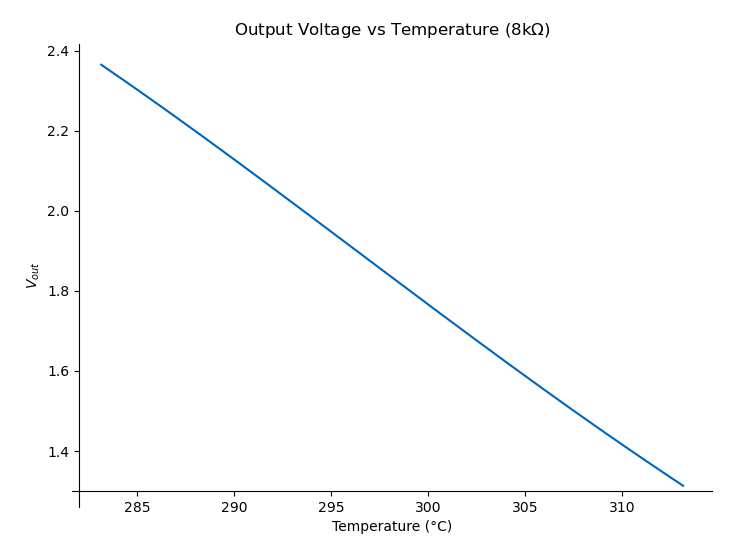
\includegraphics[width=\textwidth]{images/VoutPorTemp.png}
            \caption{ $8K\Omega$ }
        \end{subfigure}\hfill
        \begin{subfigure}{0.45\textwidth}
            \centering
            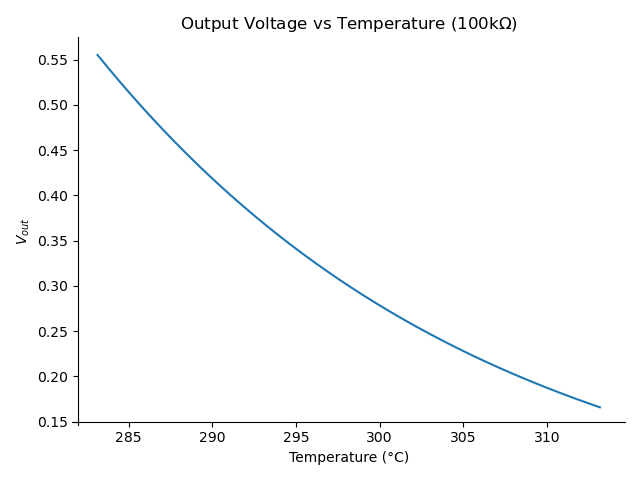
\includegraphics[width=\textwidth]{images/VoutPorTemp100k.png}
            \caption{$100K\Omega$}
        \end{subfigure}
        \caption{Output Voltage vs Temperature}
    \end{figure}

    With $R=8k$ the output signal is $V_{out} \in [1.31V;2.36V]$. 
    But the \textit{ADC} as resolution of $12$ bits and a voltage range of $3.3V$, meaning that to have the best resolution possible the signal needs an offset and a gain of $2.87$ and $-1.75$ respectively. 
    It's important to note that a $0.1V$ margin was added to $V_{out}$ in order to ensure that the \textit{AFE} works properly in the specified range.
    
    \subsubsection{Circuit Implementation}
    \label{AFENTCCirc}
    The most obvious way to achieve this values would be with a differential amplifier, 
    as seen in the following circuit.

     \begin{figure}[H] 
        \centering
        \includegraphics*[scale = 0.25]{images/AFENTCDiffAmp.png}
        \caption{NTC's AFE Differential Amplifier}
        \label{difafentc}
    \end{figure}

    Although in the simulation this yields the expected result, using the wheatstone with a precision OpAmp as bridge amplifier, it's possible to achieve gain and offset using less components, yielding better results in terms of power consumption and thermal noise. 

    
    \begin{figure}[H] 
        \centering
        \includegraphics*[scale = 0.25]{images/AFENTC.png}
        \caption{NTC's AFE topology}
        \label{AFENTC}
    \end{figure}

    As already specified the $R_3$ value is $8K~\Omega$ and for the purpose circuit dimensioning the circuit 
    the positive node of the OpAmp will be treated as a variable $V_p$.

    Using python the circuit function $V_{out}(V_p)$(see function AfeNtc() in the attached python script, script.py): 

       
    Providing the following expression:

    \begin{equation}
        V_{out} = V_p\left[ 1 + R_f\cdot\left(\frac{1}{R_1} + \frac{1}{R_2}\right) \right] - V_{cc}\cdot\frac{R_f}{R_1}
    \end{equation}

    Now it's clear to see what part of the equation is responsible for the circuit gain and offset.
    
    \begin{equation}
        \begin{cases}
            V_{offset} = - V_{cc}\cdot\frac{R_f}{R_1}\\
            G = \left[ 1 + R_f\cdot\left(\frac{1}{R_1} + \frac{1}{R_2}\right) \right]\\
        \end{cases}
    \end{equation}

    Setting $R_f = 10K$ the values that satisfy the equation system are $R_1 = 9348 \Omega$ and $R_2 = 11760 \Omega$.
    In the simulation this values are a bit too close to the limits so in order to have better margins and to use the available resistors
    the final values are  $R_1 = 9.1K \Omega$ and $R_2 = 12K \Omega$.

    The theorical output voltage of the AFE circuit in function of the temperature will have the
    following graphic.
    \begin{figure}[H] 
        \centering
        \includegraphics*[scale = 0.6]{images/outuptafentc.png}
        \caption{NTC's AFE output voltage}
        \label{NTCAFEgraph}
    \end{figure}

    From this graphic, the maximum and minimum voltages values can be extracted, so from them, the output voltage 
    will vary between $V_{outAFE} \in [0.15V;3.25V]$, from 10ºC to 40ºC, theoretically. These values are within the \textit{ADC} range, so no information will be lost.
\subsection{LM35}

    This integrated-circuit temperature sensor, generates an output
    voltage linearly proportional to the Centigrade temperature.

    $$V_{out} = 10^{-2}\cdot T$$

    Hence, in the specified conditions $V_{out}\in[0.1;0.4]$. 
    To increase resolution as done in \hyperref[AFENTCCirc]{NTC's AFE subsection},
    it's needed to add gain and an offset. 
    For this purpose a differential amplifier can be used.  
    
    \begin{figure}[H] 
        \centering
        \includegraphics*[scale = 0.3]{images/DiffAmpLM35.png}
        \caption{LM35 Differential Amplifier.}
        \label{difafelm}
    \end{figure}

    Although this circuit achieves the expected output, the amount of components,
    increases noise and power consumption, thus the used topology was a non-inverting amplifier.

    \begin{figure}[H] 
        \centering
        \includegraphics*[scale = 0.2]{images/AFELM35.png}
        \caption{AFE for the LM35 sensor.}
        \label{AFELM35}
    \end{figure}

    This way the input impedance is high, only one OpAmp and two resistors are used.
    But this comes with the cost of lost resolution. With a gain of $7.8$ $V_{out}\in[0.78V,3.12V]$
    $0.78V$ or $23.6\%$ of range in the \textit{ADC} are lost.

    Graphically, the output voltage of the LM35 AFE is the following.

    \begin{figure}[H] 
        \centering
        \includegraphics*[scale = 0.5]{images/Outafelm35.png}
        \caption{LM35 AFE output voltage.}
        \label{AFELM35graph}
    \end{figure}
\subsection{Power Consumption}

    In modern electronic systems, power consumption plays a crucial role. This section analyzes the power consumption of the temperature meter system as a whole.
    So in order to determine the total power consumption, the power of all the resistances present in both AFE circuits were considerd and the theorical 
    typical consumption of the OpAmps, resulting in the next equation.
    
    \begin{equation}
        P_{total} =  P_{AFENTC} + P_{AFELM35}[W] 
    \end{equation}
    Where
    \begin{equation}
        P_{AFENTC} = \frac{(V_{CC} - V_{NTC})^2}{R_1} + \frac{(V_{CC} - V_{NTC})^2}{R_3} + \frac{V_{NTC}^2}{R_2} + \frac{(V_{NTC} - V_{Out_{AFENTC}})}{R_5} + I_{OpAmp} \cdot V_{CC} [W]
    \end{equation}
    And
    \begin{equation}
        P_{AFELM35} = \frac{(V_{LM35} - V_{Out{AFELM35}})^2}{R_b} + \frac{V_{LM35}^2}{R_a} + I_{OpAmp} \cdot V_{CC} [W]
    \end{equation}
    
    The total power will depend on the temperature on a second degree function, since the voltage function by temperature is a first degree, after the linearisation.
    The power consumption graphic for each AFE circuit are the following.

    \begin{figure}[h]
        \centering
        \begin{subfigure}{0.45\textwidth}
            \centering
            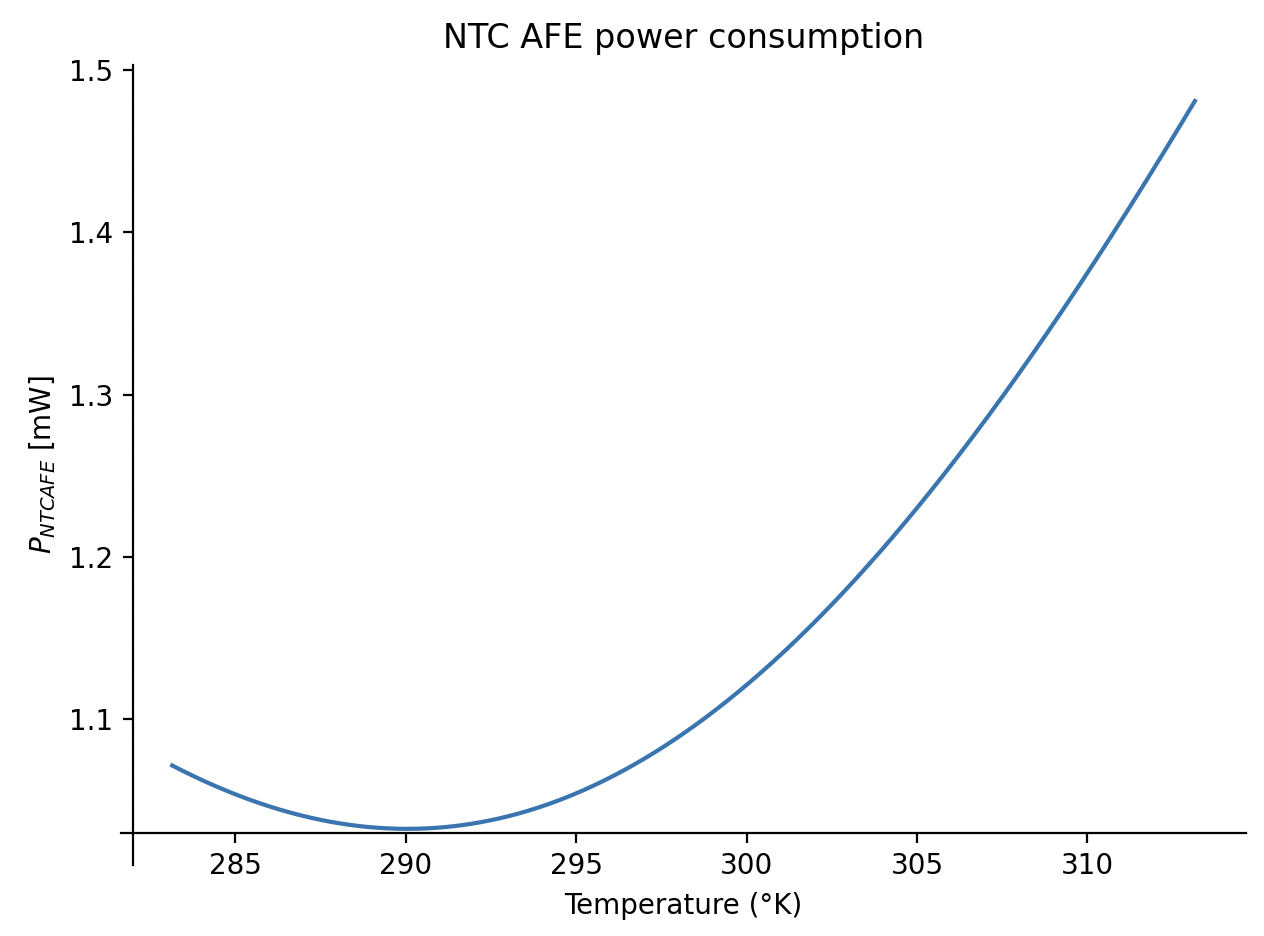
\includegraphics[width=\textwidth]{images/PowerNTC.png}
            \caption{ NTC }
        \end{subfigure}\hfill
        \begin{subfigure}{0.45\textwidth}
            \centering
            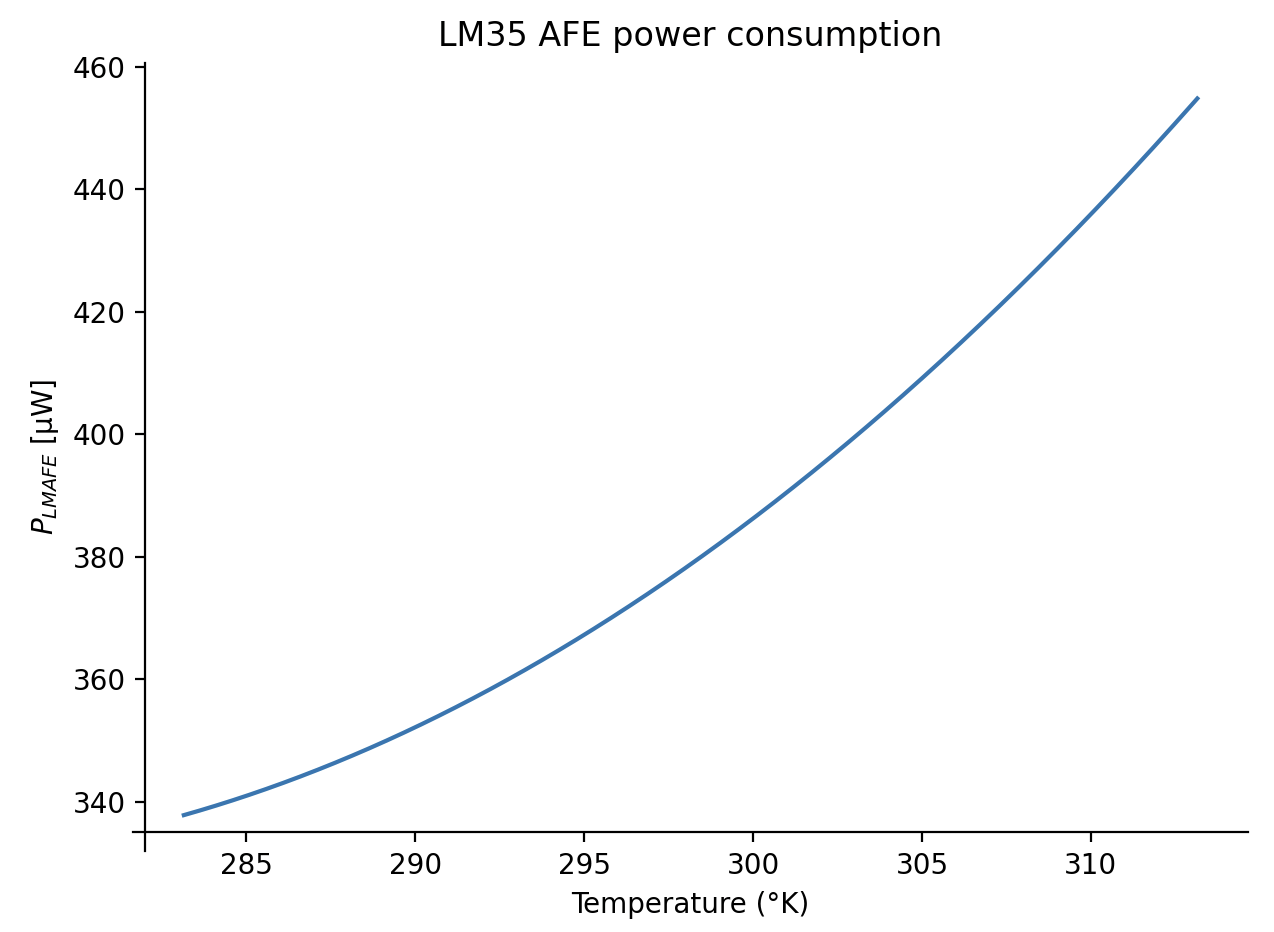
\includegraphics[width=\textwidth]{images/PowerLM.png}
            \caption{ LM35 }
        \end{subfigure}\
        \begin{subfigure}{0.45\textwidth}
            \centering
            \includegraphics*[scale = 0.35]{images/PowerTotal.png}
            \caption{Total power consumption.}
        \end{subfigure}
        \caption{NTC and LM35 AFEs power consumption.}
        \label{powerteo}
    \end{figure}

    \begin{comment}
    
    The total power consumption graphic is then.
    \begin{figure}[H] 
        \centering
        \includegraphics*[scale = 0.5]{images/PowerTotal.png}
        \caption{AFEs total power consumption.}
    \end{figure}

    \end{comment}
    
    From the graphic above, the power consumption describes a parabolic, where the value of the power consumption increases with the 
    temperature, with a maximum value of $P_{total} = 1.93 mW$. So, both circuits delivered satisfactory results in this regard, 
    especially, the LM35 AFE circuit, where the consumption was in the order of the microWatts.
\subsection{Output Relay }
    
    Lastly the \textit{MCU} will turn on and off a fan. For this purpose 
    a relay will open and close the fan circuit. Because the \textit{MCU's I/O} 
    can't drive the relay a \textit{NPN} transistor is use to get enough current.
    Thus the following circuit also needs to be dimensioned. It's important to note
    that the diode is needed to protect the circuit.
    
    \begin{figure}[H] 
        \centering
        \includegraphics*[scale = 0.4]{images/RelayDrive.png}
        \caption{Relay circuit.}
        \label{relaycircuit}
    \end{figure}

    The voltage supply value for this circuit must be different form the AFE circuits that were presented,
    since the minimum supply voltage to operate the relay is $5V$. And for this voltage, the 
    current on the inductor present in the relay is $72mA$, according to the datasheet.
    
    So, considering $V_{BE} = 0.7V$, and $\beta = 150$ the equation to define the resistance of this circuit is the next.
    \begin{equation}
        R = \frac{I/O_{HIGH}-V_{BE}}{I_r}\cdot \beta\\
        \Leftrightarrow R = 5416.(6) \Omega
    \end{equation}

    The closest value available and the final value of this resistance will be $R = 5.1 k\Omega$.
\newpage
\section{Simulations}
\subsection{NTC}
    
    For the purpose of testing the following circuit was designed.
    At first with linear voltage supply since as seen in \hyperref[AFENTCOutV]{NTC's AFE} section, this voltage is almost linear.

    Producing the following results.
 
    \begin{figure}[H] 
        \centering
        \includegraphics*[scale = 0.3]{images/NTCLinearRes.png}
        \caption{Linear supply NTC test results.}
        \label{wrap-fig:1}
    \end{figure}

    Confirming the effectiveness of the \textit{AFE} circuit a more realistic
    circuit was then tested.

    \begin{figure}[H] 
        \centering
        \includegraphics*[scale = 0.6]{images/NTCRealTb.png}
        \caption{Realistic NTC test circuit.}
        \label{wrap-fig:1}
    \end{figure}
    
    With the following results.
    
    \begin{figure}[H] 
        \centering
        \includegraphics*[scale = 0.3]{images/NTCRealRes.png}
        \caption{Realistic NTC test results.}
        \label{wrap-fig:1}
    \end{figure}

    Comparing both results the difference is minimal. Confirming that the output is nearly linear in relation to the temperature variation.
    
    \begin{figure}[H] 
        \centering
        \includegraphics*[scale = 0.3]{images/NTCRealLinearComp.png}
        \caption{NTC Linear and Realistic results comparison.}
        \label{wrap-fig:1}
    \end{figure}


\subsection{LM35}

    For this sensor the simulation is straight forward, since the output is linear and proportional to the temperature, 
    it can be simulated with a variable voltage supply. 
    
    The circuit used to test was the same seen in the \hyperref[AFELM35]{lm35 design section}.
    Giving the following results, confirming that this approach works as expected. 
    
    \begin{figure}[H] 
        \centering
        \includegraphics*[scale = 0.15]{images/LM35AFERes.jpeg}
        \caption{LM35 AFE test results.}
        \label{LM35AFERes}
    \end{figure}

\subsection{Monte-Carlo Analysis} 
    
    The Monte-Carlo simulation is needed for the sake of testing our circuits resilience to resistor variation, considering 
    the normal distribution of those values. 

    This values can be found on the following interval.
    \begin{equation}
        R_{real} \in [R_{ideal} - tol; R_{ideal} + tol] 
    \end{equation}
    Where the variable \textit{tol} will depend with the serie of resistances used. 
    In this work, the serie used is the E12, with a maximum tolerance of 5\%. So to test the results of
    the output of the two AFE circuits, one hundred simulations were made to assure the reliability of the normal distribution.

    The results for the NTC AFE are the following.

    \begin{figure}[H]
        \centering
        \includegraphics*[scale = 0.3]{images/montecarlo ntc.png}
        \caption{NTC AFE Monte-Carlo test results}
        \label{montecarlontc}
    \end{figure}

    And the results for the LM35 AFE circuits.

    \begin{figure}[H]
        \centering
        \includegraphics*[scale = 0.3]{images/montecarlo lm35.png}
        \caption{LM35 AFE Monte-Carlo test results}
        \label{montecarlolm}
    \end{figure}

    By analysing the results of the Monte-Carlo simulation of the NTC AFE, first of all, we can conclude that the
    slope of the output voltage will be almost the same, the only difference will be in the offset of this function.
    This variation on the offset will unfortunately alter the final result for all temperatures, but the maximum deviation is just  $3^\circ C$, in a worts case scenario.

    One other implication of this offset is the values for lower temperatures, where the output would be greater than $3.3V$, so the OpAmp will saturate and the voltage will stay at $3.3V$.

    For the results of the LM35 AFE Monte-Carlo test, the biggest difference between the thirty simulations is the slope of the output voltage,
    because the resistances in this circuit only affects it's gain. This consequence is more problematic at higher temperatures, since the input voltage is greater at this values.

    To better visualize the variation in the output voltage of both systems at the maximum, minimum and average temperature, a more specific simulation was used, where the value of the $R_{NTC}$ and the
    $V_{LM35}$ were fixed for the temperature tested.
    So first of all, for 10ºC, the results are represented in figure \ref{10ºC - montecarlo}.

    \begin{figure}[H]
        \centering
        \begin{subfigure}{0.45\textwidth}
            \centering
            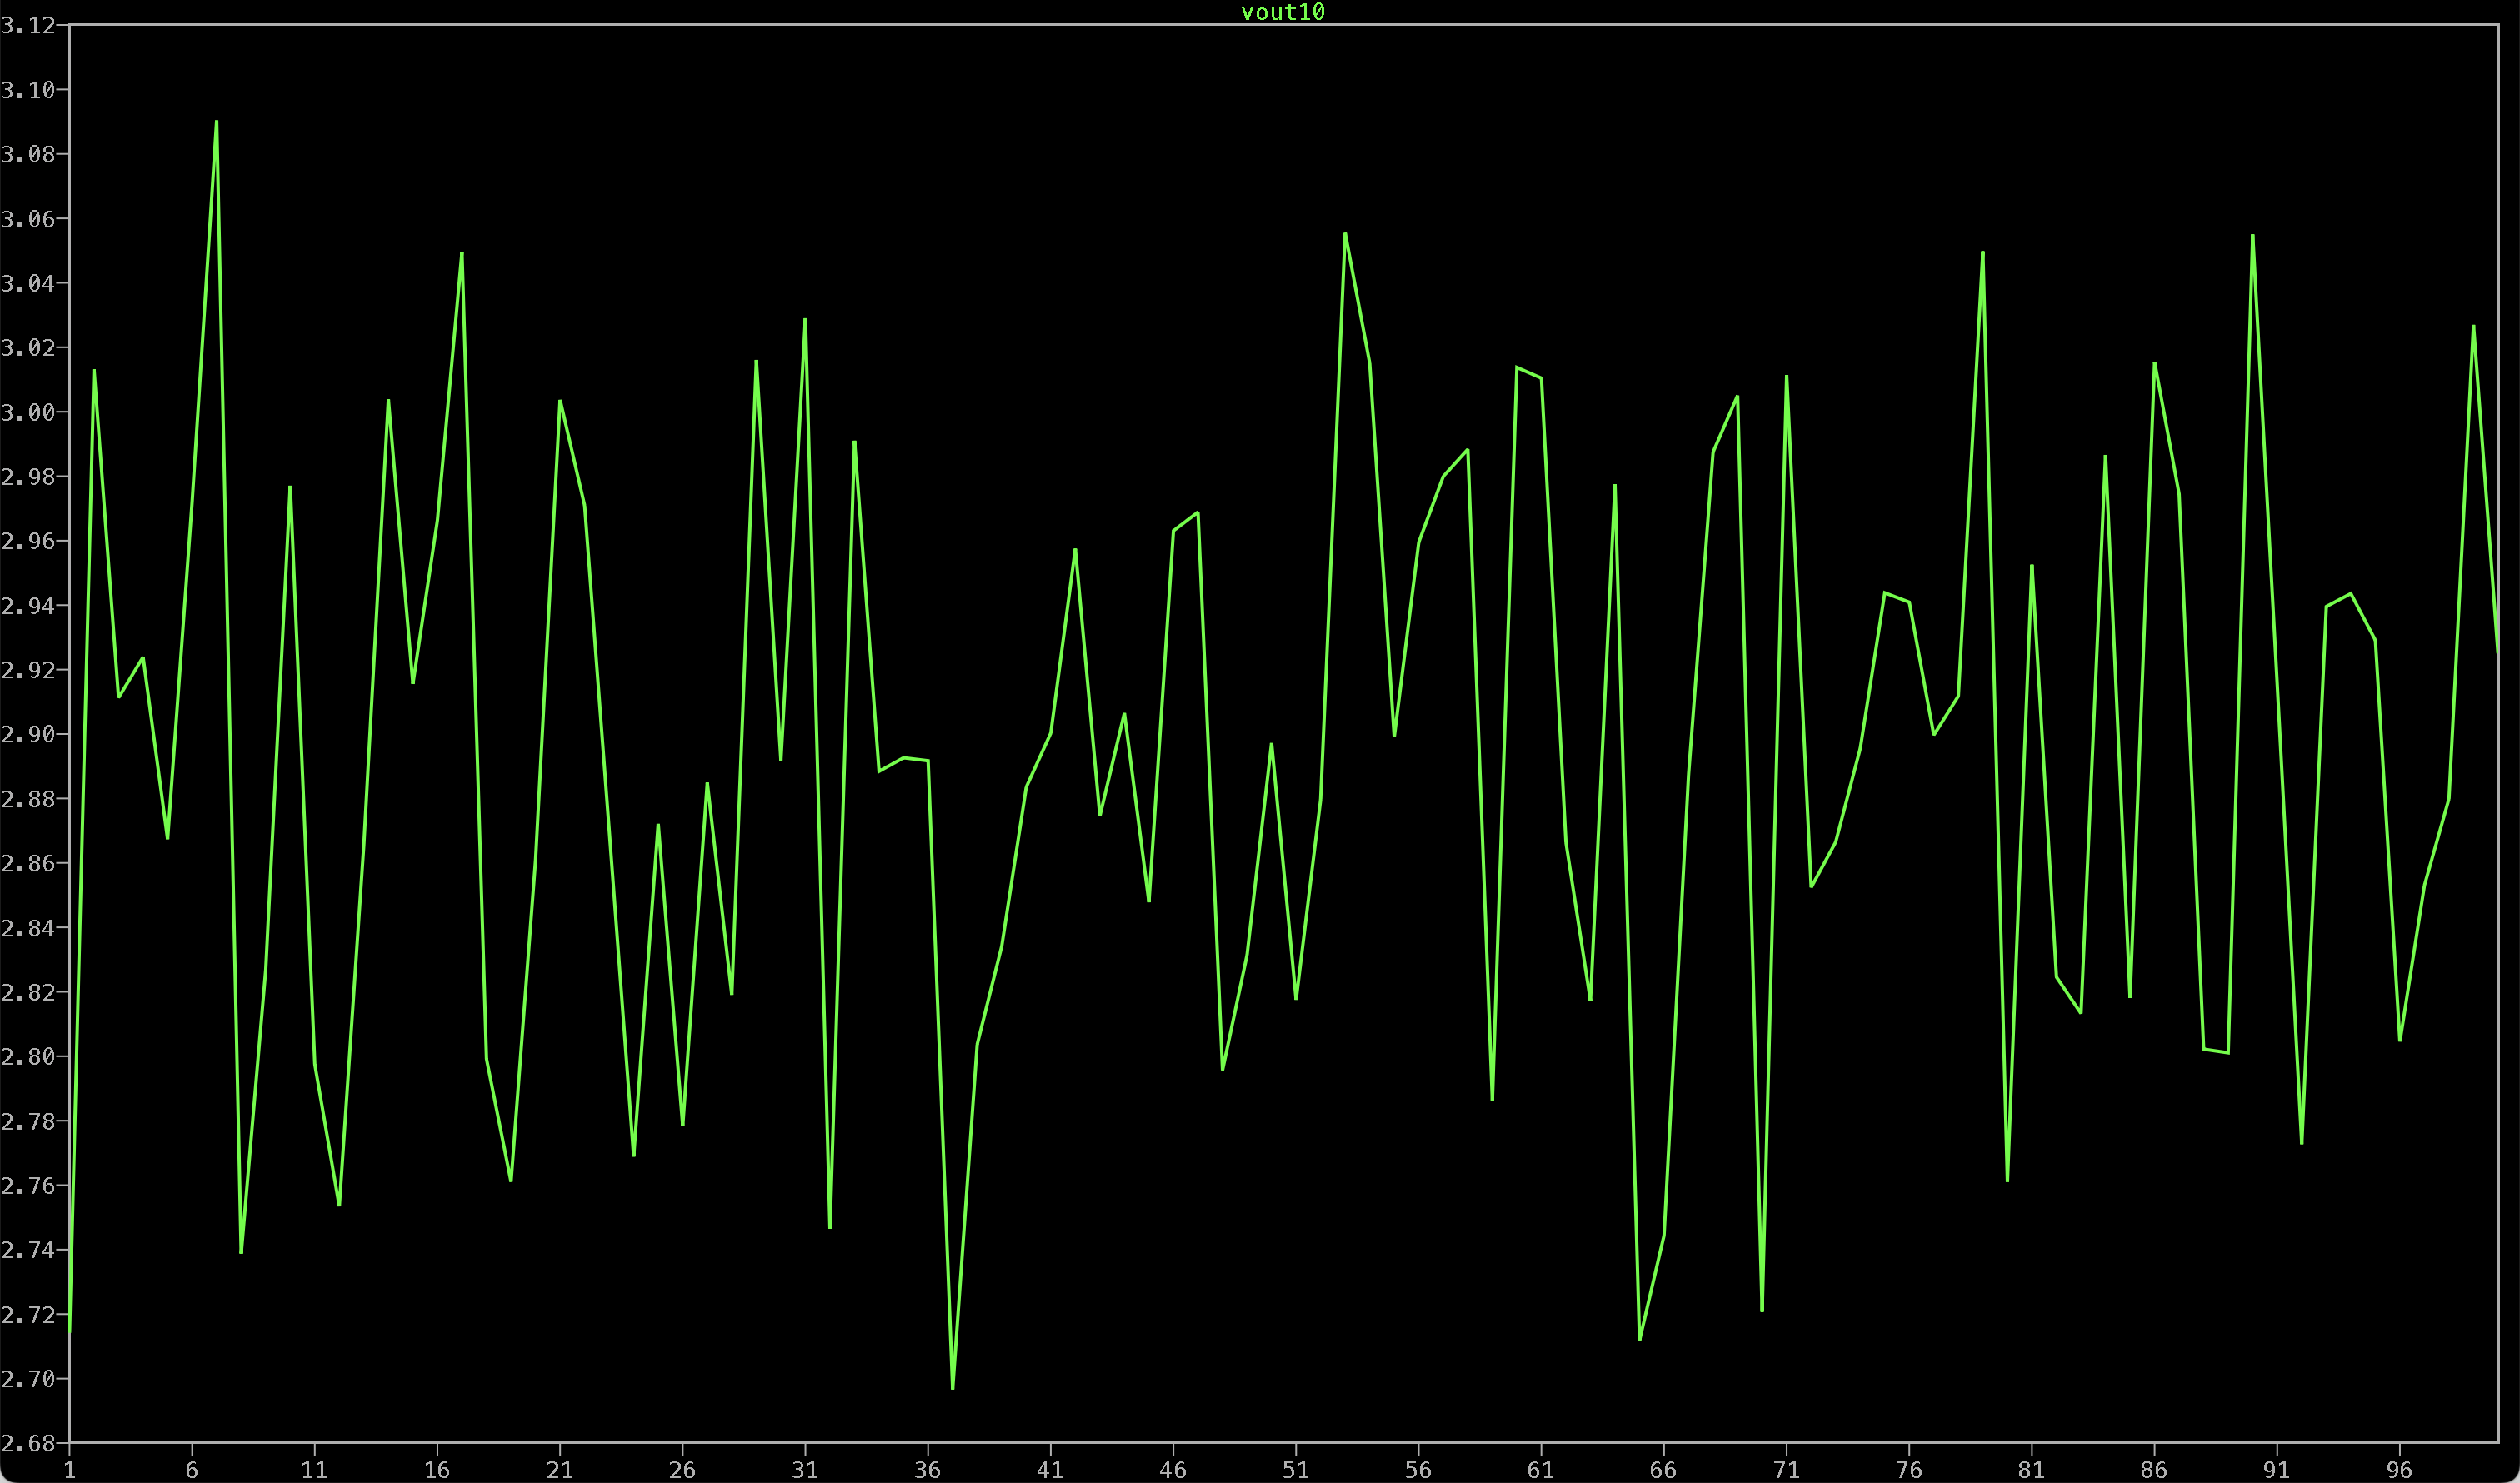
\includegraphics[width=\textwidth]{images/vntc10.png}
            \caption{ $V_{OutAFENtc}$ }
        \end{subfigure}\hfill
        \begin{subfigure}{0.45\textwidth}
            \centering
            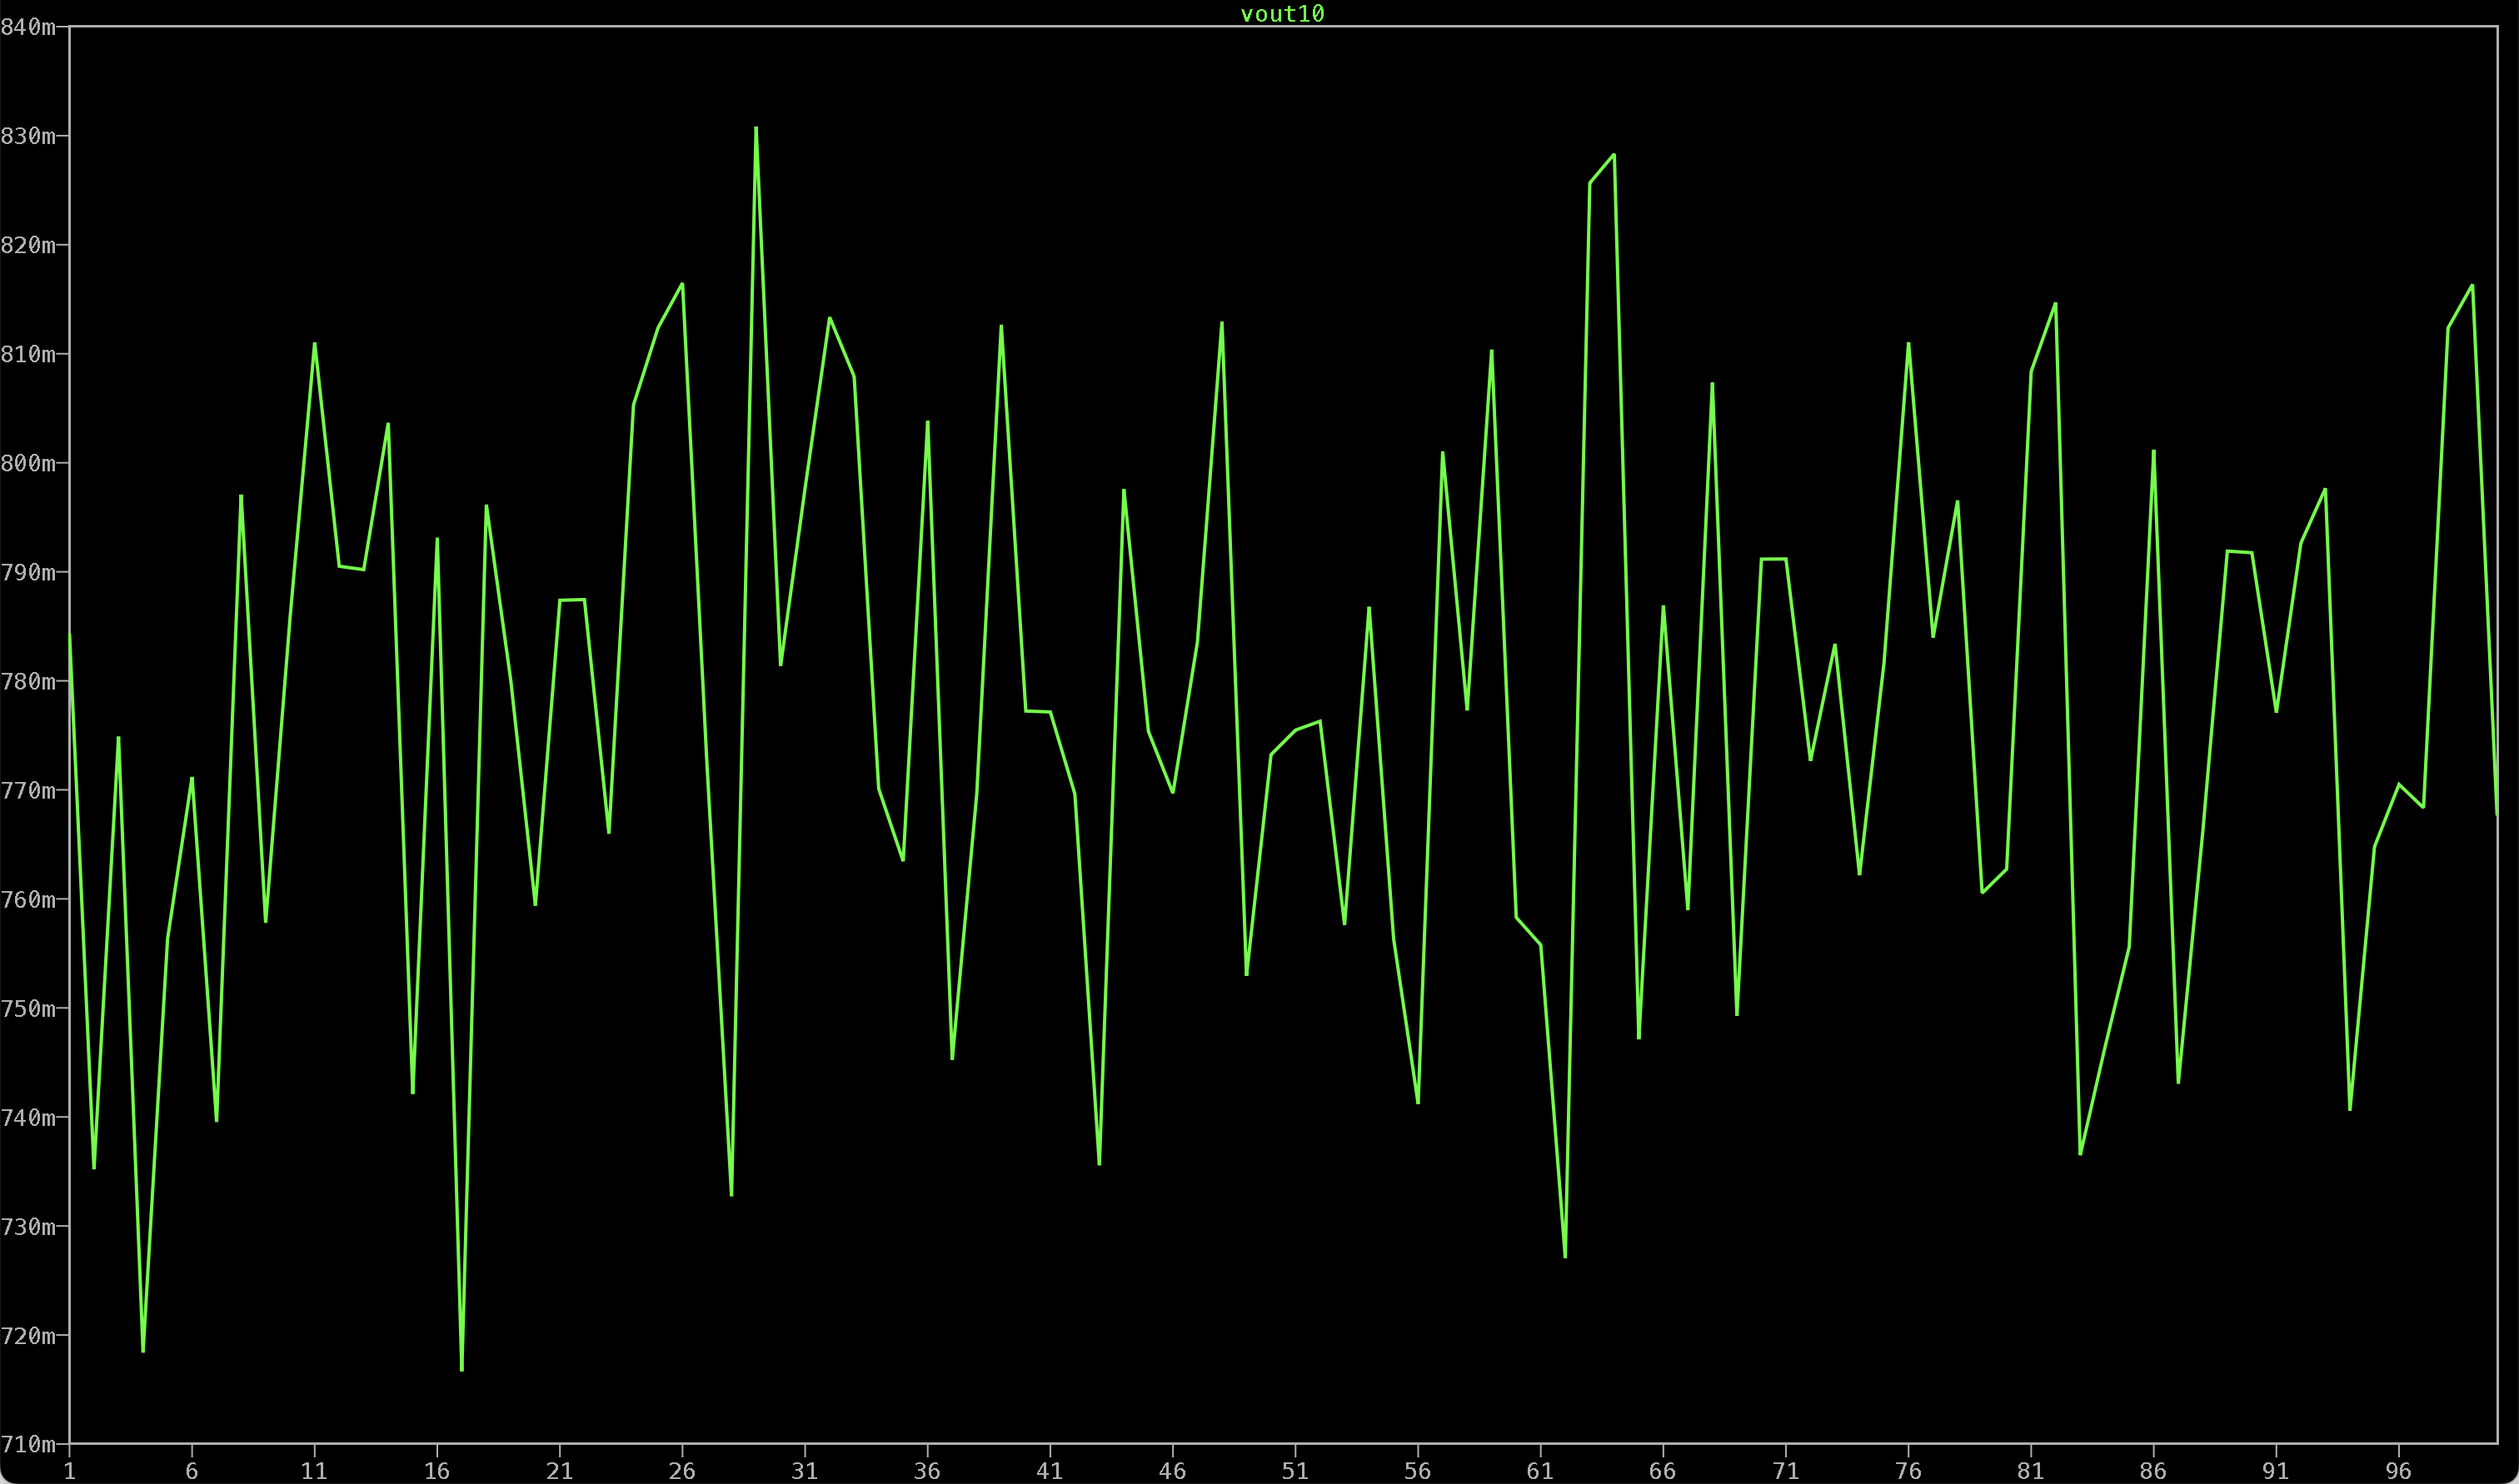
\includegraphics[width=\textwidth]{images/vlm10.png}
            \caption{$V_{OutAFELm35}$}
        \end{subfigure}
        \caption{Output Voltage variations at 10ºC}
        \label{10ºC - montecarlo}
    \end{figure}

    For 25ºC, in figure \ref{25ºC - montecarlo}.

    \begin{figure}[H]
        \centering
        \begin{subfigure}{0.45\textwidth}
            \centering
            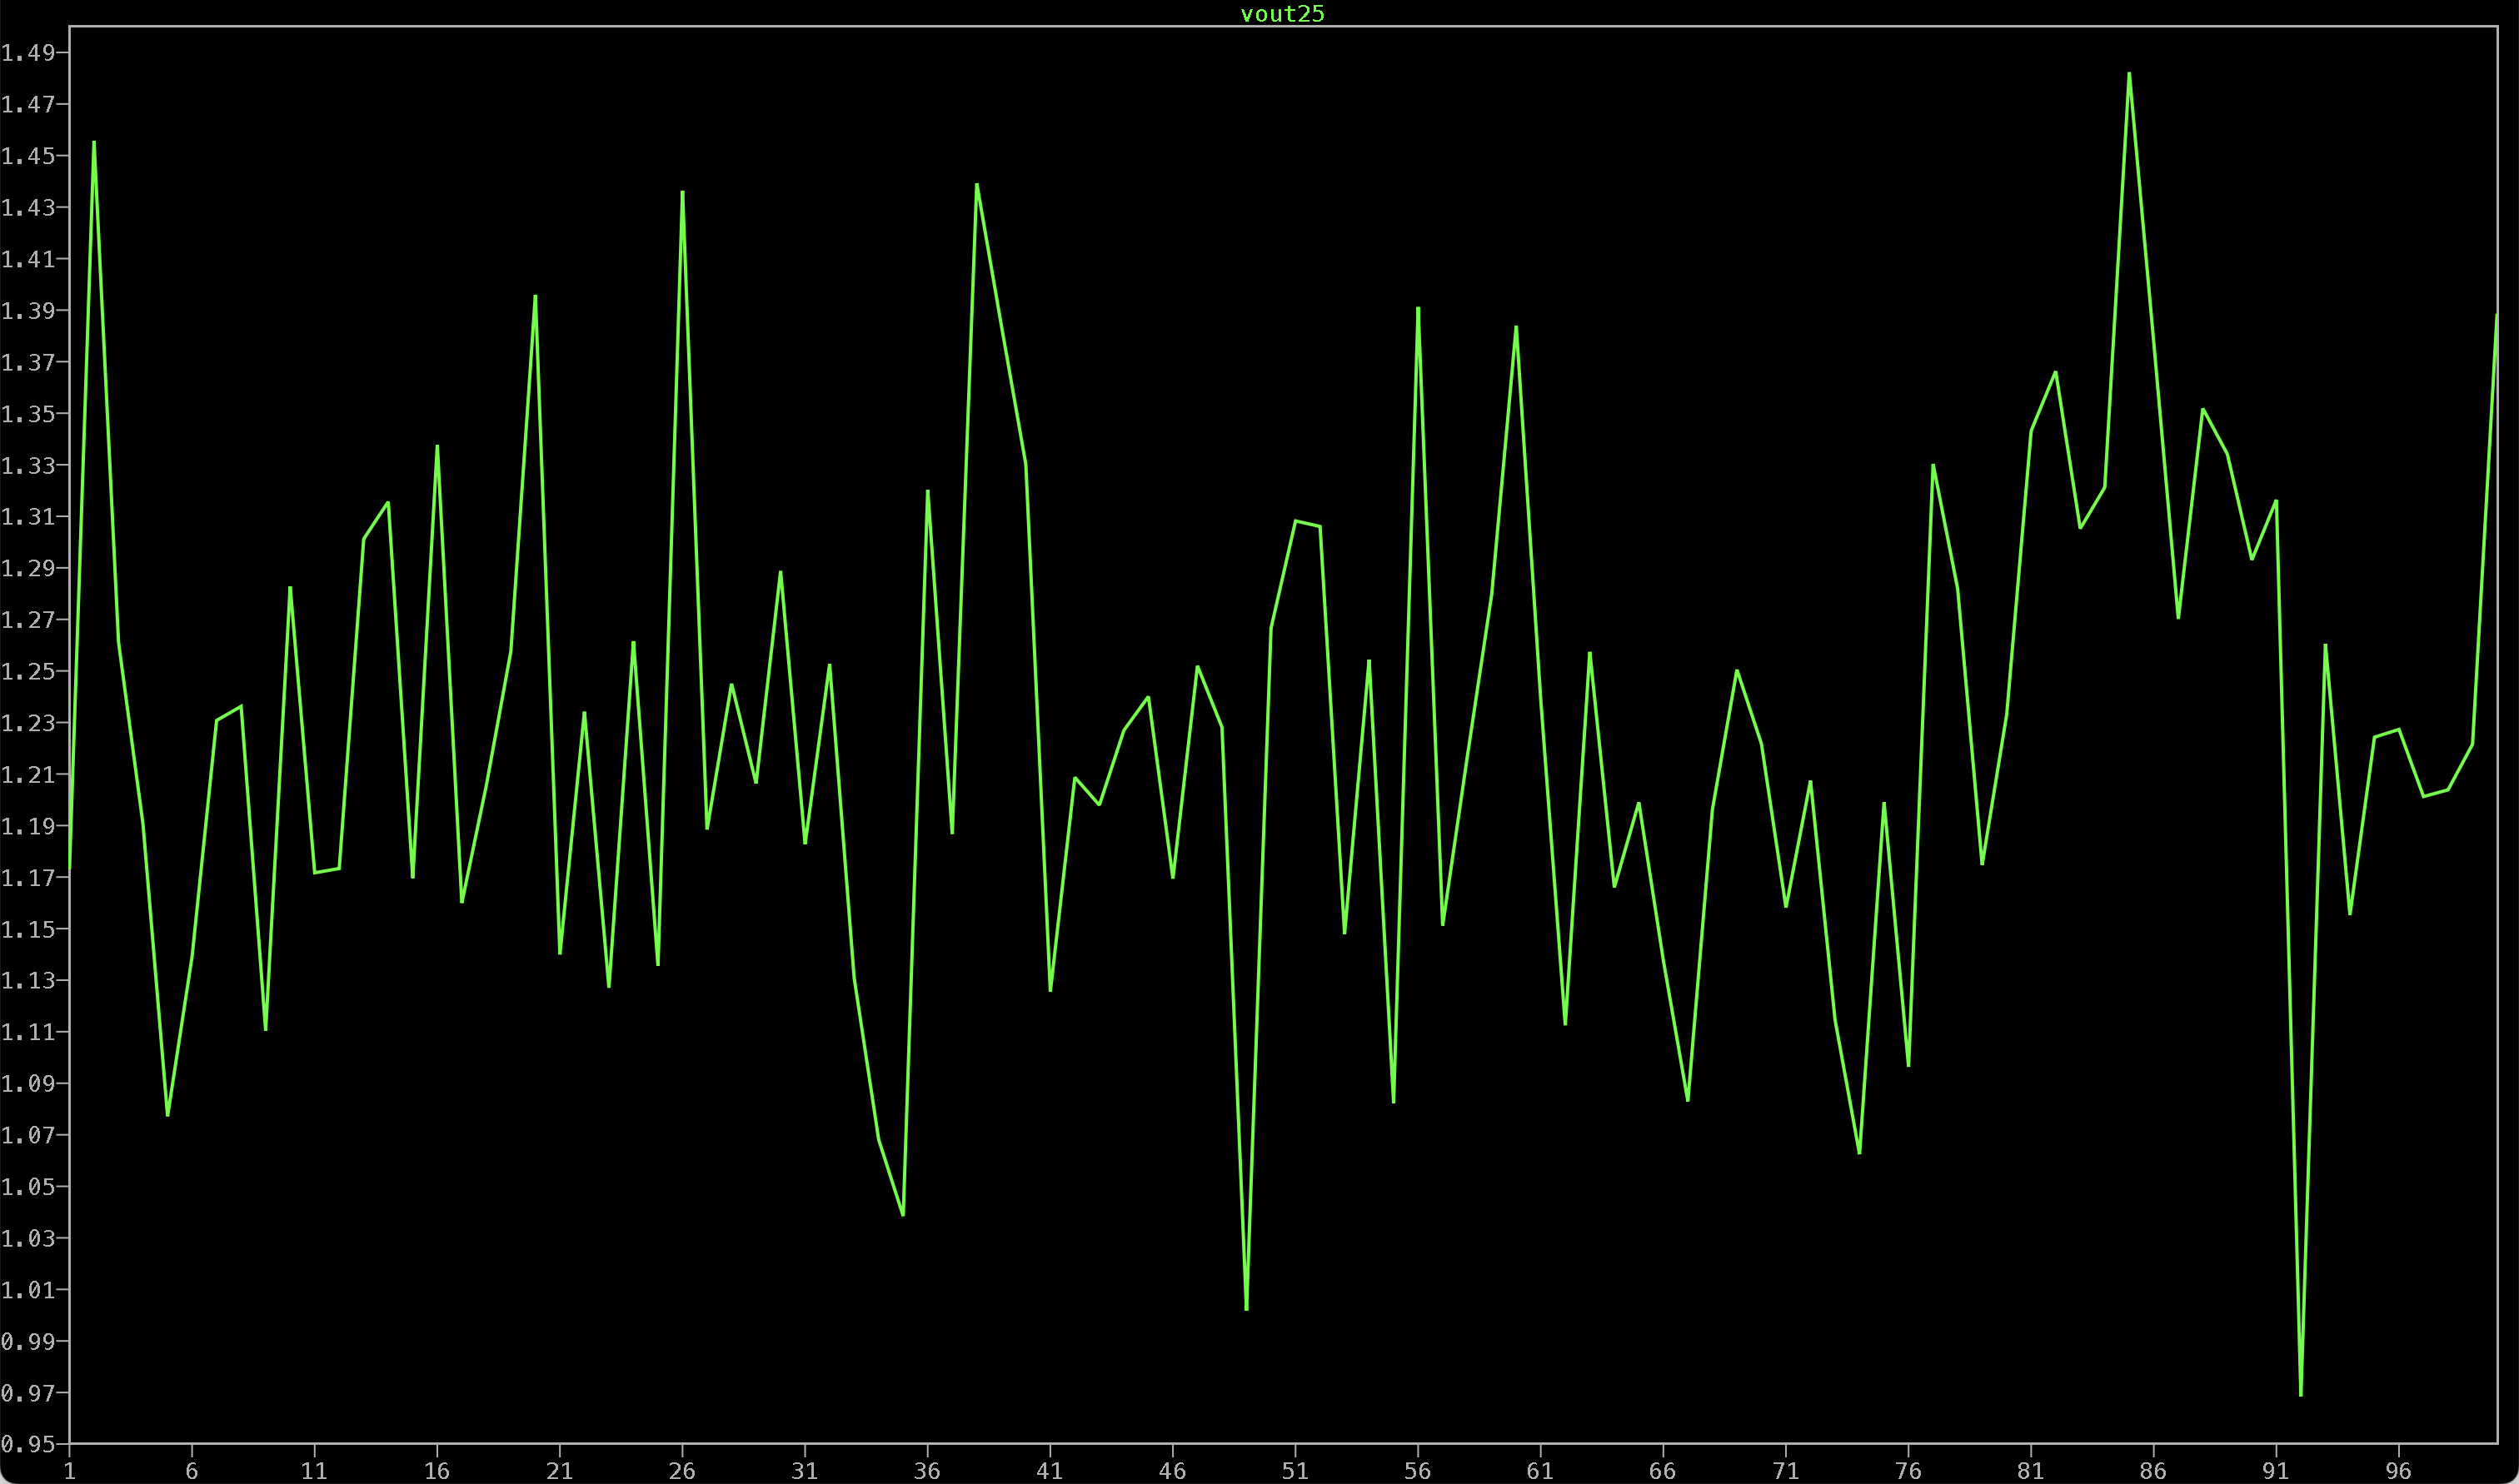
\includegraphics[width=\textwidth]{images/vntc25.png}
            \caption{ $V_{OutAFENtc}$ }
        \end{subfigure}\hfill
        \begin{subfigure}{0.45\textwidth}
            \centering
            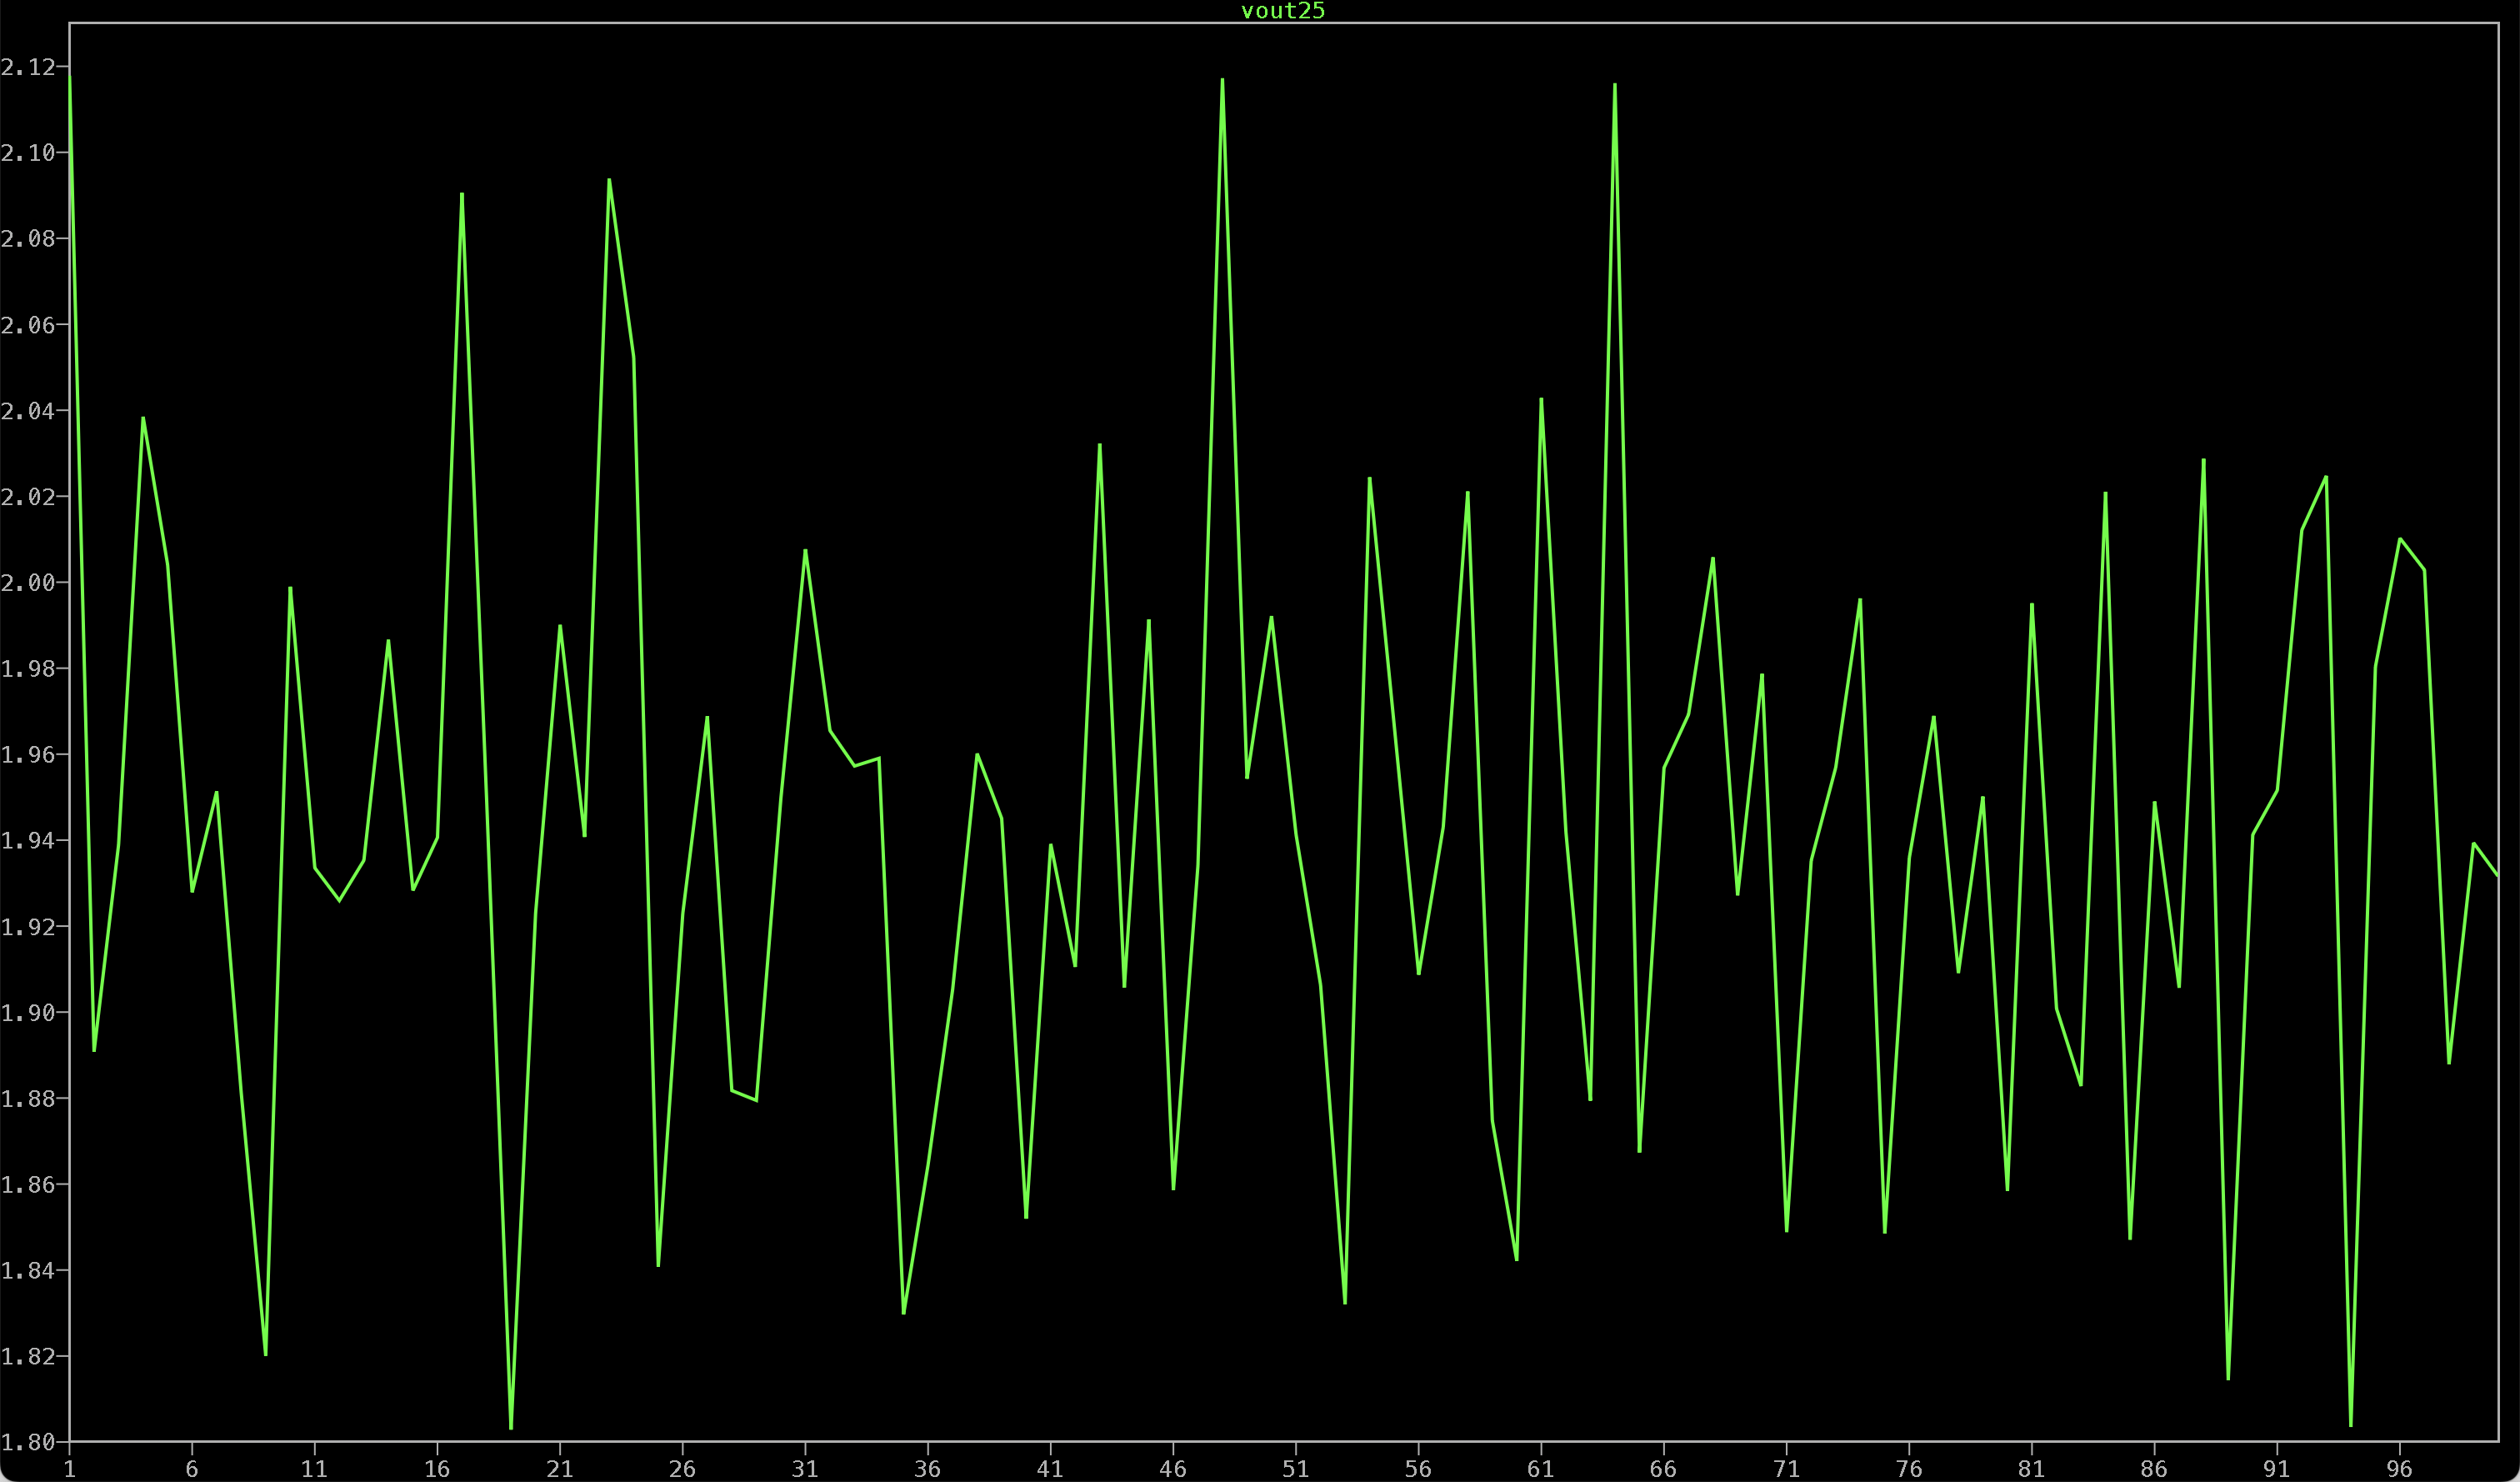
\includegraphics[width=\textwidth]{images/vlm25.png}
            \caption{$V_{OutAFELm35}$}
        \end{subfigure}
        \caption{Output Voltage variations at 25ºC}
        \label{25ºC - montecarlo}
    \end{figure}

    And finally, for the maximum temperature of 40ºC, the results are shown in figure \ref{40ºC - montecarlo}

    \begin{figure}[H]
        \centering
        \begin{subfigure}{0.45\textwidth}
            \centering
            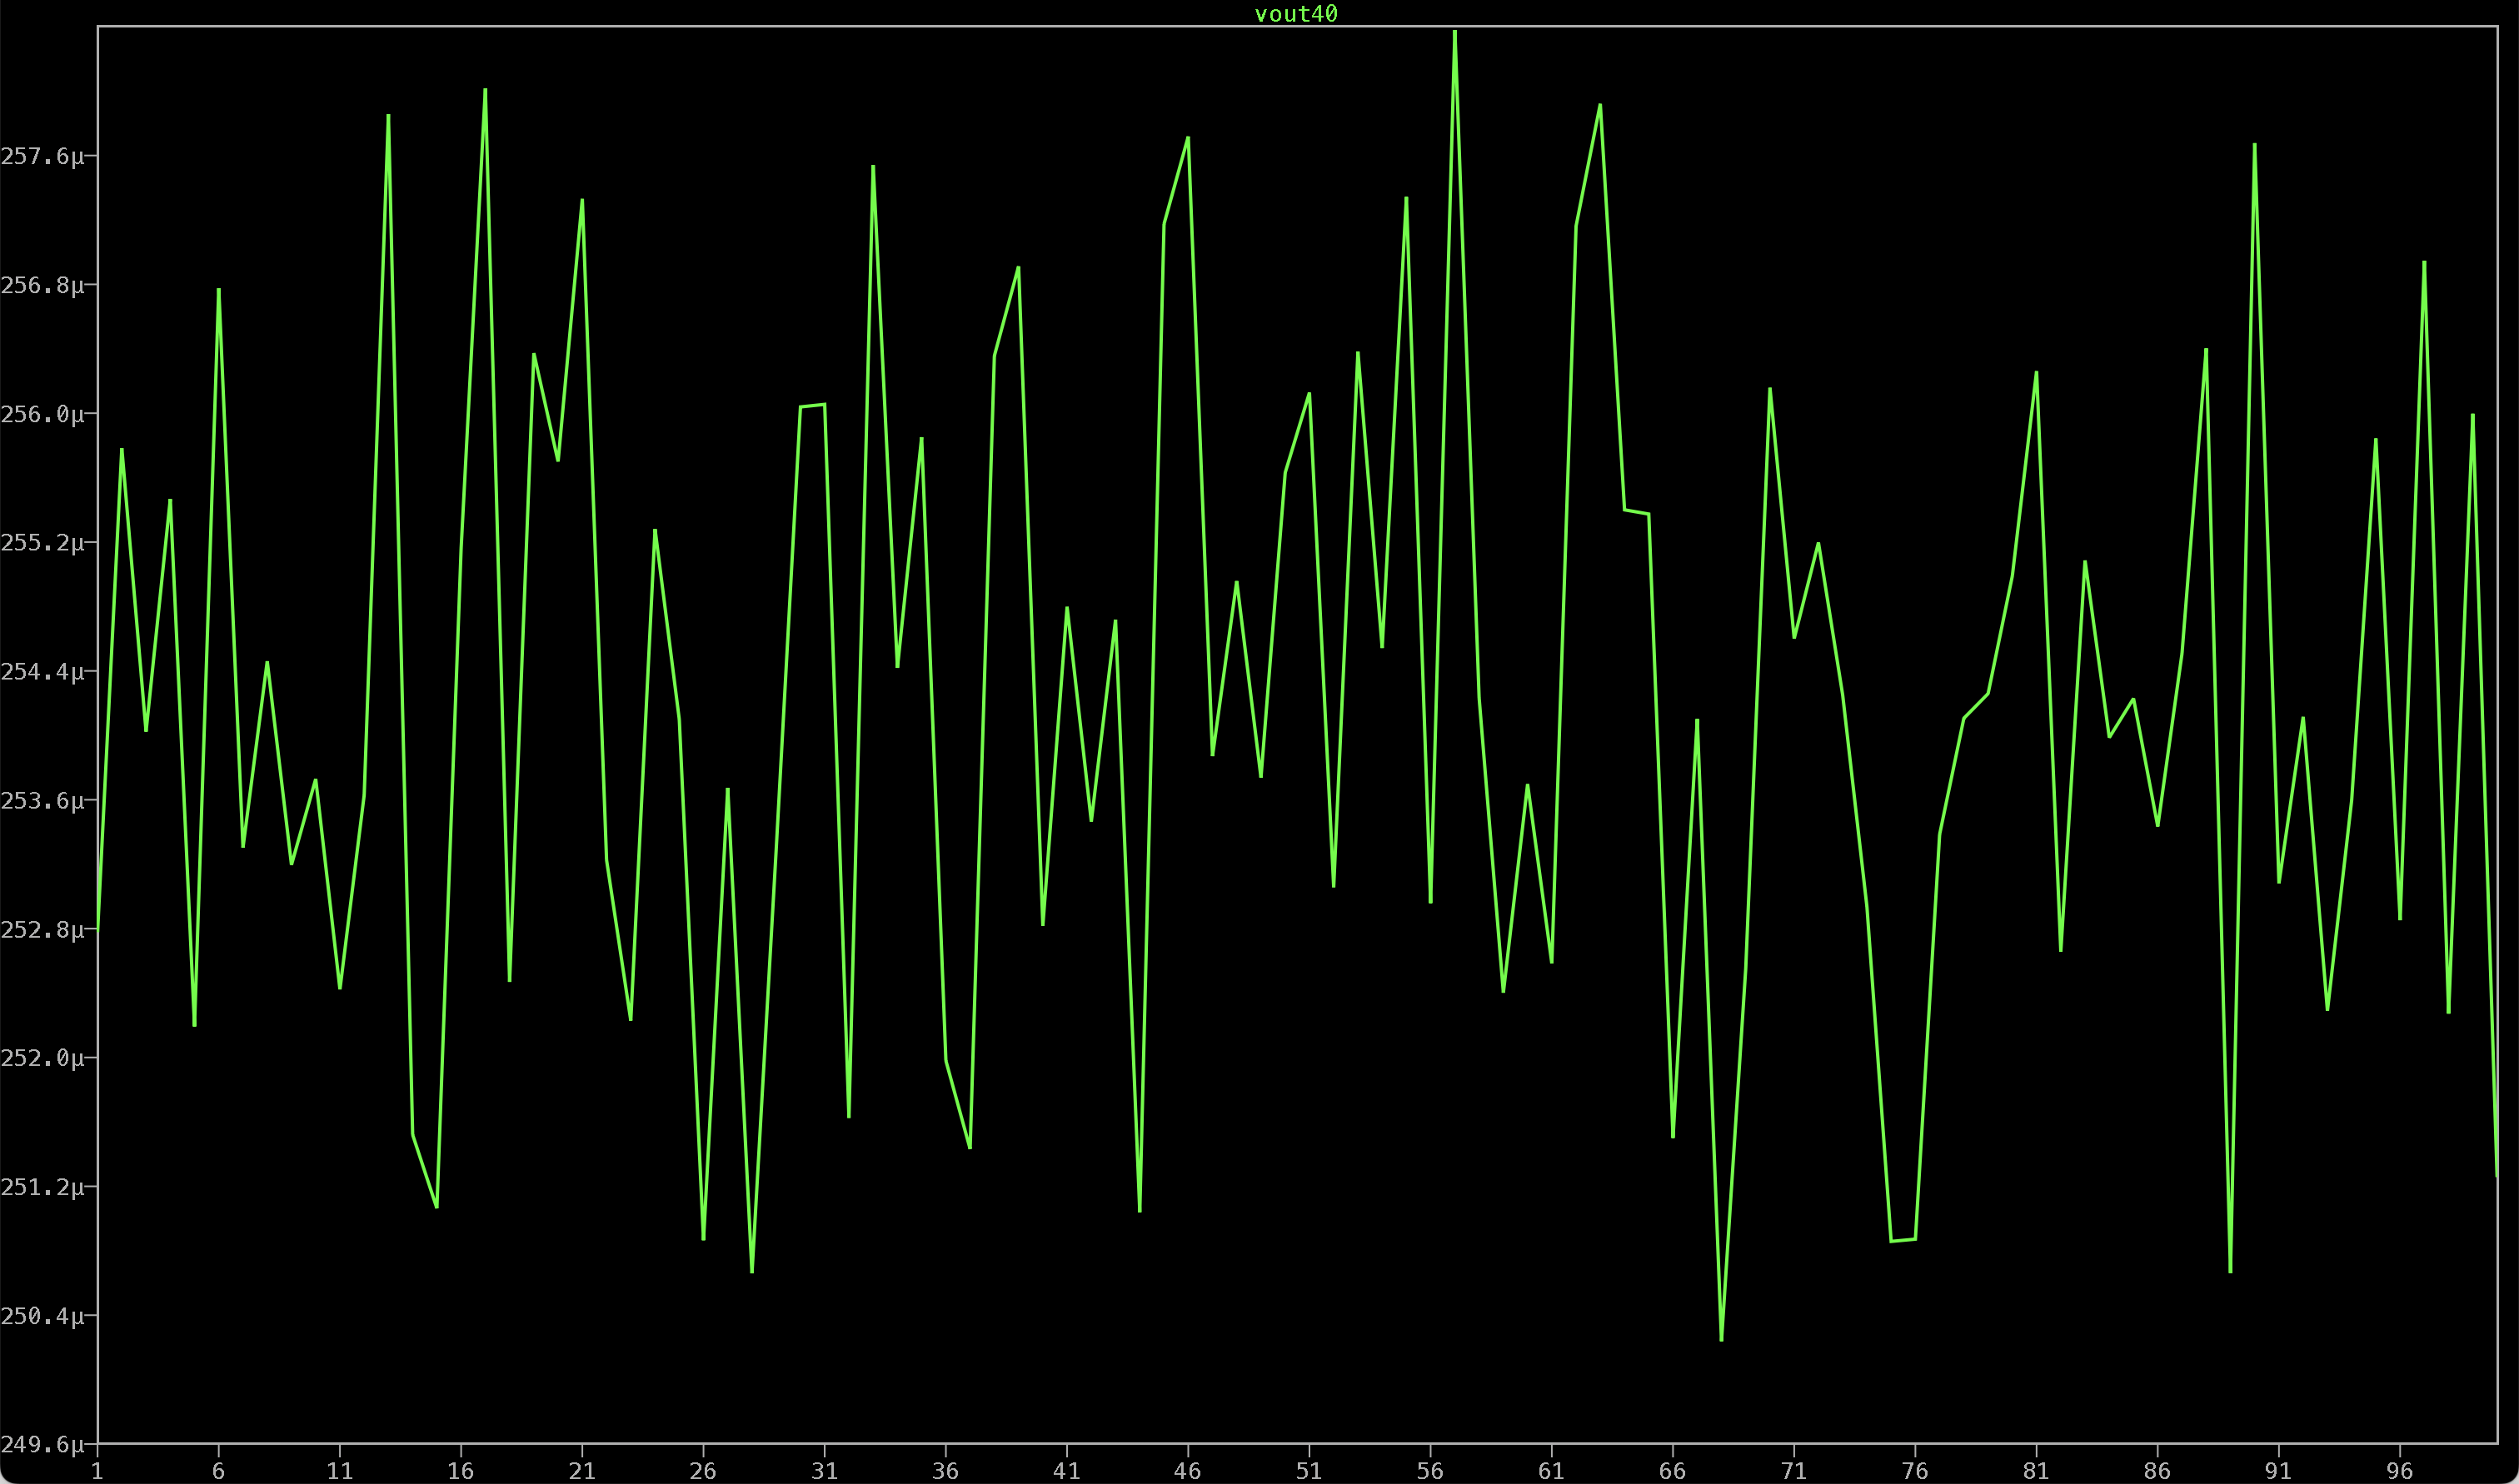
\includegraphics[width=\textwidth]{images/vntc40.png}
            \caption{ $V_{OutAFENtc}$ }
        \end{subfigure}\hfill
        \begin{subfigure}{0.45\textwidth}
            \centering
            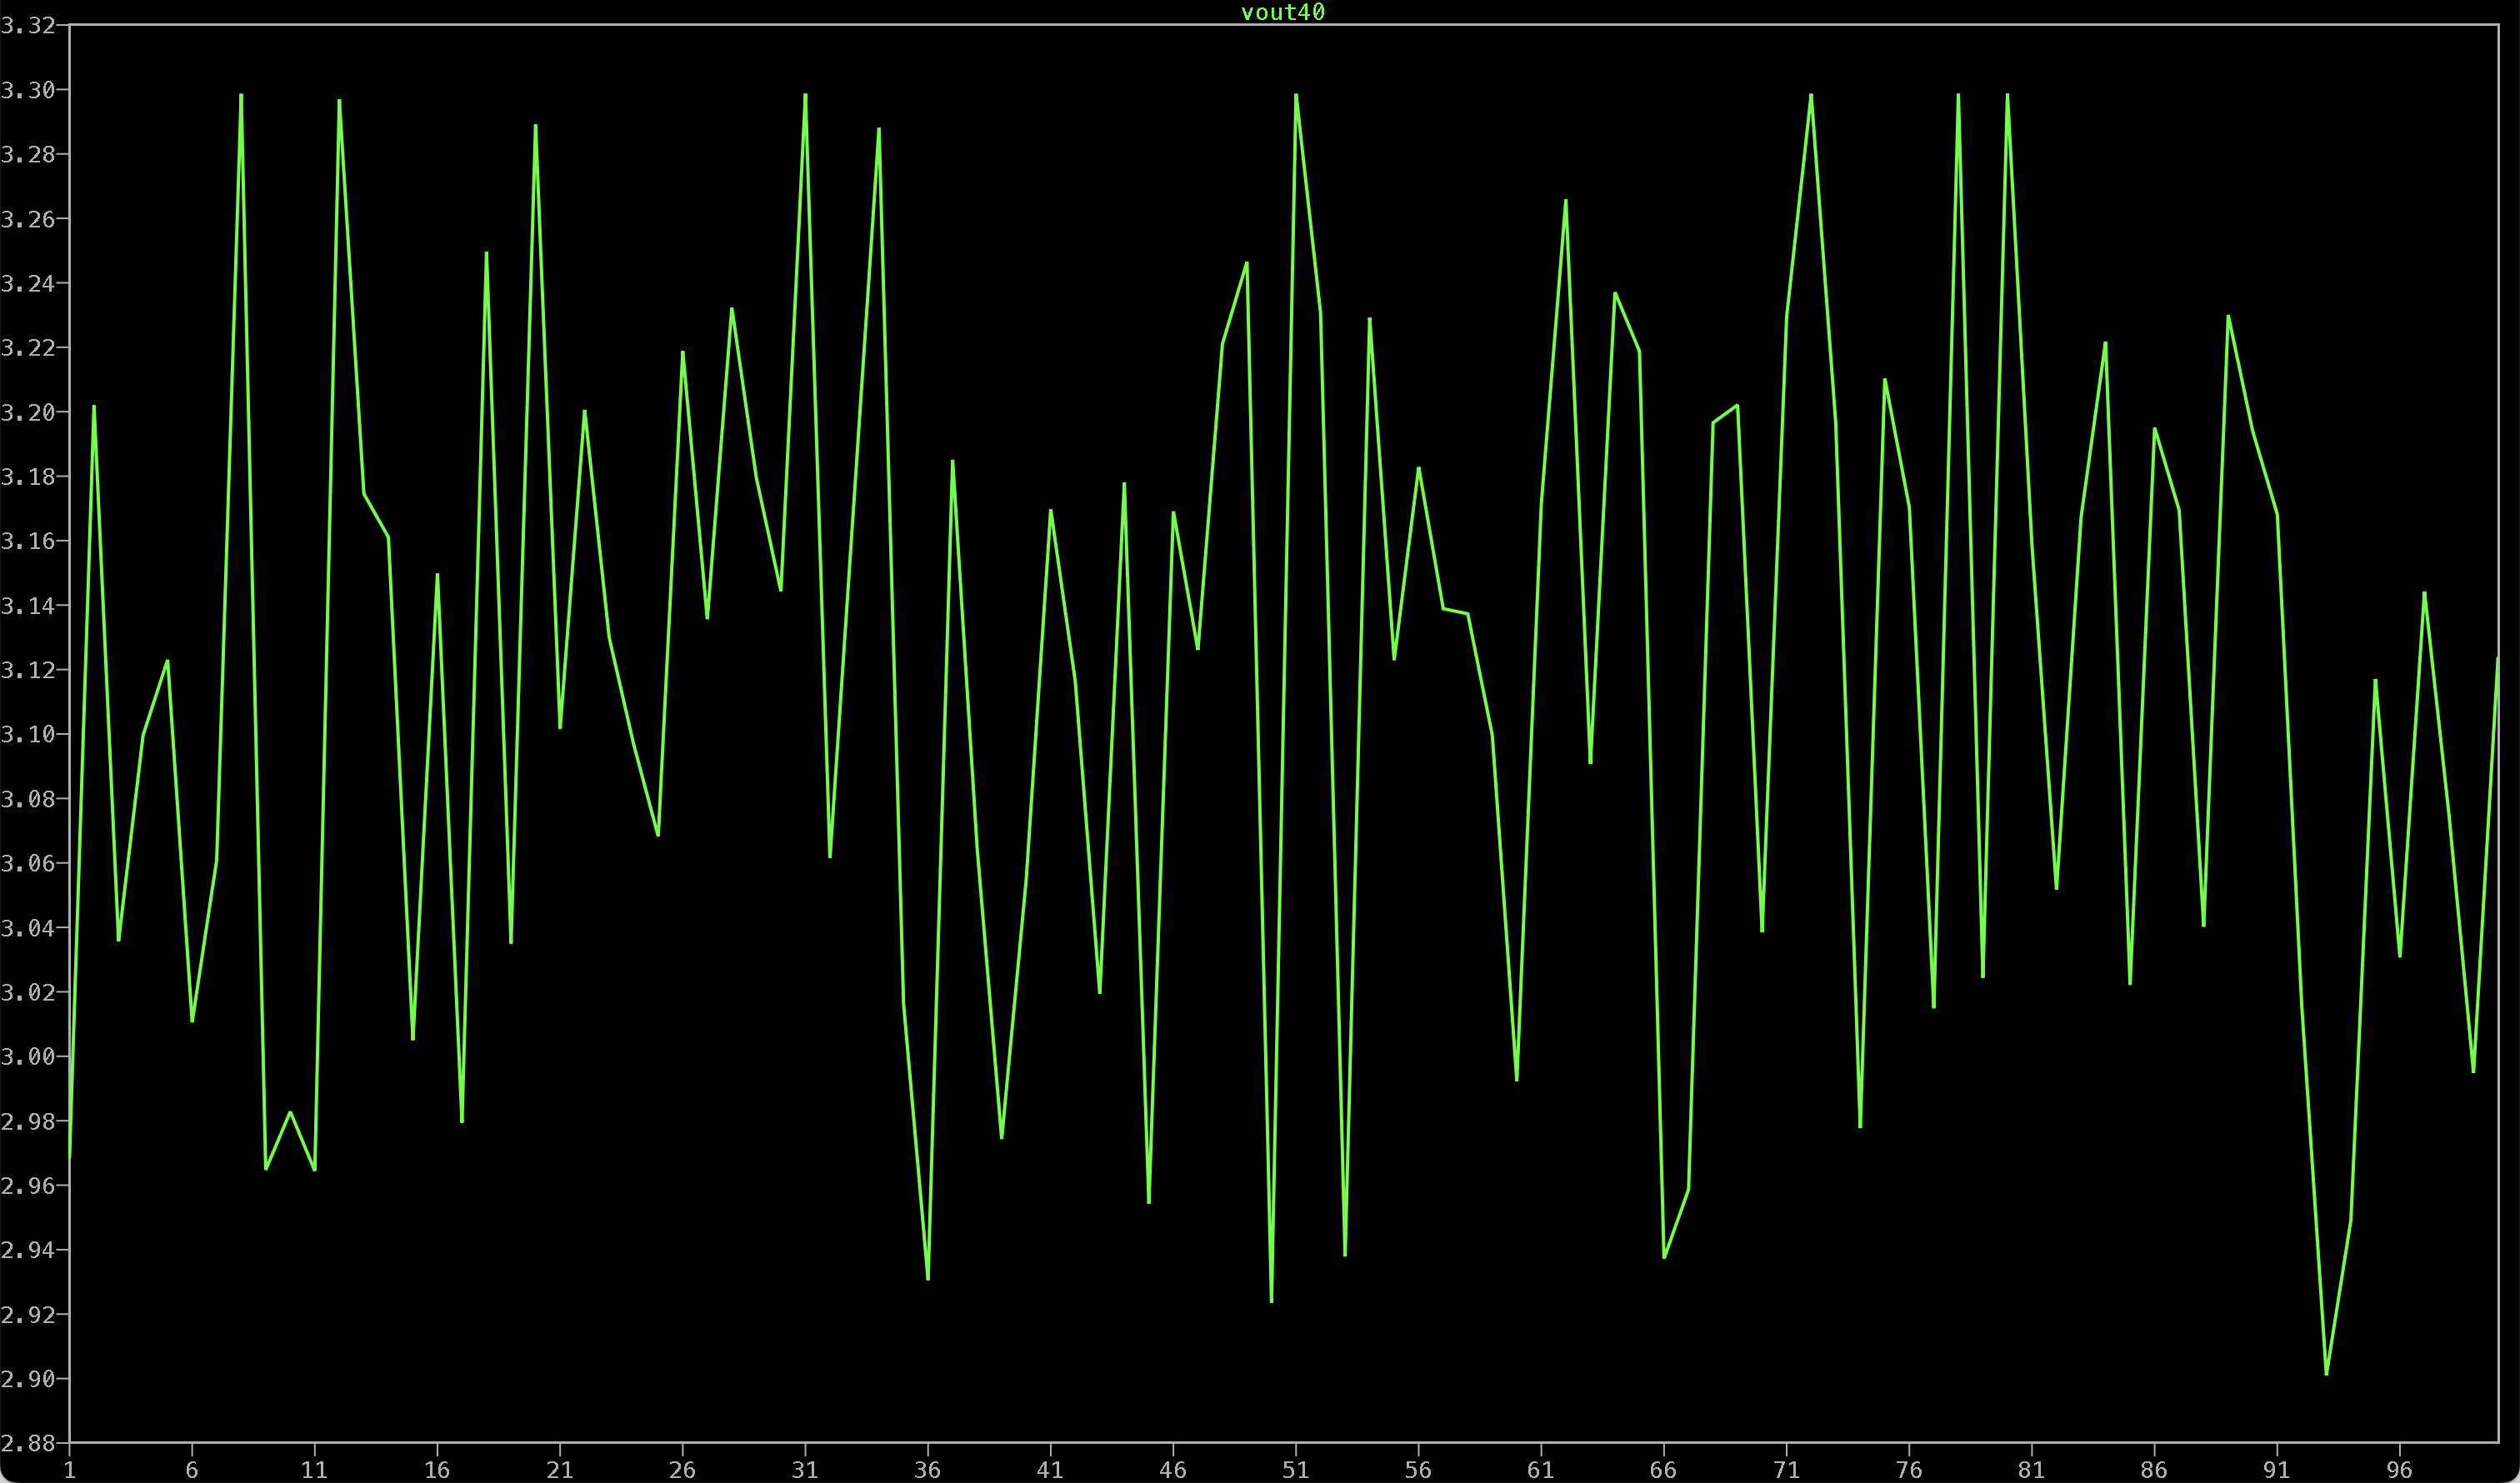
\includegraphics[width=\textwidth]{images/vlm40.png}
            \caption{$V_{OutAFELm35}$}
        \end{subfigure}
        \caption{Output Voltage variations at 40ºC}
        \label{40ºC - montecarlo}
    

    \end{figure}
    
    By analysing the previous figures, the hypothesis presented before about the variations in the output voltage being related with the 
    temperature in the LM35 AFE is confirmed,
    but another conclusion may also be taken, the higher the voltage, higher the variation of this value.

    \subsection{Power Consumption}
    
    In LTSpice, in order to determine the total power consumption of both AFE circuits, we only need to check the power of the voltage supply.
    Yielding the following results, represented in figure \ref{powersim}.
        
    \begin{figure}[H] 
        \centering
        \includegraphics*[scale = 0.3]{images/PowerConsumption.png}
        \caption{System Power Consumption.}
        \label{powersim}
    \end{figure}

    The power consumption increases with temperature, confirming the theoretical values obtained earlier, but the curve described is not a parabola, despite presenting a similar form. After analysing the power consumption of each device, the conclusion was that the OpAmp present in the NTC's AFE had a different behavior from the expected, where instead of having a constant consumption, it presented the behavior represented in the figure \ref{OpAmpNTC}.
 
    \begin{figure}[H] 
        \centering
        \includegraphics*[scale = 0.3]{images/PowerAmpop.png}
        \caption{OpAmp NTC AFE Power Consumption.}
        \label{OpAmpNTC}
    \end{figure}

    This behavior will not affect negatively the final implementation of the circuit, although the power consumption of the simulated system was slightly above the expected, the maximum value reached the $2.37mW$, instead of the $1.93mW$ theoretically calculated.
    
\section{Implementation and Experimental Tests}

In this section the implementation of the system will be described, as well as the results obtained from the experimental tests. For the implementation of the circuit was used an MCU, the ESP32, and the software used was the PlatformIO. The code used for the implementation of the system can be found in the attached files.

\subsection{Circuit Implementation}

As shown in  Figure \ref{fig:circuit-implementation}, the circuit was implemented using the components described in the previous sections. The circuit was powered by the ESP32, with a voltage of $3.3V$. 

The relay was used to mimic the control of a fan, and the sensors were connected to the AFE circuits if needed. The outputs of the sensors were connected to the ADC of the ESP32, and the results were displayed on the GUI.
\begin{figure}[H] 
    \centering
    \includegraphics*[scale = 0.09]{images/circuit_implementation.png}
    \caption{Circuit Implementation.}
    \label{fig:circuit-implementation}
\end{figure}

The pins used in the ESP32 can be found in Table \ref{tab:pins}.


\begin{table}[h]
    \centering
    \caption{ESP32 Pins used in the circuit.}
    \begin{tabularx}{\textwidth}{>{\centering\arraybackslash}X >{\centering\arraybackslash}X >{\centering\arraybackslash}X >{\centering\arraybackslash}X}
        \toprule
        \textbf{Signal} & \textbf{Pin name} & \textbf{Pin mode}\\
        \midrule
        $V_{out}$ LM35 AFE & D2 & ADC2\_2 (INPUT)\\
        \midrule
        $V_{out}$ NTC AFE & D4 & ADC2\_0 (INPUT)\\
        \midrule
        $Digital_{out}$ DS18B20 & D5 & GPIO 5 (INPUT)\\
        \midrule
        $Digital_{in}$ Relay & D18 & GPIO 18 (OUTPUT)\\
        \bottomrule
    \end{tabularx}
    \label{tab:pins}
\end{table}


\subsubsection{DS18B20 circuit}

For the implementation of the DS18B20 sensor, a $4,7K\Omega$ pull-up resistor was used as suggested in the datasheet\textsuperscript{\cite{DS18B20_datasheet}} shown in Figure \ref{fig:ds-block-diagram}. The sensor was connected to the ESP32, and the results were displayed on the GUI. 

\begin{figure}[H] 
    \centering
    \includegraphics*[scale = 0.4]{images/Ds_block_diagram.png}
    \caption{DS18B20 block diagram.}
    \label{fig:ds-block-diagram}
\end{figure}

\subsubsection{By-pass Capacitors}

In order to reduce the noise in the ESP32 ADC, bypass $0,1\mu C$ capacitors were used. The capacitors were connected between the ADC input pads and the ground.

The ESP32 ADC is susceptible to high-frequency noise from various sources (e.g., switching power supplies, nearby electromagnetic interference)\textsuperscript{\cite{ESP-IDF-Programming-Guide}}. A bypass capacitor can short these high-frequency noise signals to ground, preventing them from reaching the ADC as a result the ADC reads a cleaner, more stable voltage signal, leading to more accurate conversions.

In this case, the capacitor acts like a low-pass filter: it allows the low-frequency (DC) signal, which is what is being measured, to pass through, but it blocks high-frequency noise by absorbing it. Thus, the ripple is reduced in the voltage being read by the ADC, minimizing noise-related fluctuations.

\subsubsection{D2 switch}
Due to design constraints, the D2 or GPIO 2 pin of the ESP 32 was used to read the output of the LM35 AFE. This pin as a particularity, it is a strapping pin, which means that it is used to put the ESP32 into bootloader or flashing mode\textsuperscript{\cite{ESP-IDF-Programming-Guide}}.

In order to avoid conflict in serial communications, a switch was added to the circuit, so that the pin could be used to read the output of the LM35 AFE, and then be disconnected when the ESP32 was being flashed or boot mode. 

\subsection{Software}
The software was developed using C++ and Python. The C++ code was used to program the ESP32, and the Python code was used to develop the GUI. The code used for the implementation of the system can be found in the attached files.

In Figure \ref{fig:flowchart} is shown a flowchart of the software implementation. The ESP32 reads the output of the sensors, and then sends the data to the GUI. The GUI displays the data in real-time, and the user can control the fan using the GUI.

\begin{figure}[H] 
    \centering
    \includegraphics*[scale = 0.8]{images/jpoliveira.jpg}
    \caption{Flowchart of the software implementation.}
    \label{fig:flowchart}
\end{figure}

The interface was developed using the Tkinter library, which is a standard Python interface to the Tk GUI toolkit. The Tkinter library is easy to use and allows for the creation of simple and intuitive interfaces. In Figure \ref{fig:gui} is shown the GUI developed for the system.

\begin{figure}[H] 
    \centering
    \includegraphics*[scale = 0.4]{images/GUI-presentation.png}
    \caption{GUI developed for the system.}
    \label{fig:gui}
\end{figure}

\subsubsection{Multisampling}

In order to improve the accuracy of the temperature readings, a multisampling technique was used. The ESP32 reads the output of the sensors multiple times and then calculates the average value. This technique helps to reduce noise and improve the accuracy of the temperature readings.

\subsection{Experimental Tests}

    The experimental tests were conducted to evaluate the performance and accuracy of the temperature sensing system. The primary objective was to verify the functionality of the three different sensors—NTC thermistor, LM35, and DS18B20—and compare their responses under controlled temperature changes.

    To simulate real-world temperature variations, the sensors were placed together in close proximity, and hot air was used to gradually heat them. This method allowed us to observe how each sensor responded to increasing temperatures in real time and to measure the accuracy of the readings obtained from the ESP32's ADC. The system's outputs were displayed on the graphical user interface (GUI), providing a direct comparison between the temperature readings from the different sensors.

        
    \subsubsection{ Sensors }

        Firstly we test without changing the temperature, this way the difference between readings is more obvious.
        
        \begin{figure}[H] 
            \centering
            \includegraphics*[scale = 0.5]{images/TempFixTest.png}
            \caption{Sensor readings for fix temperature.}
            \label{fig:FixTemp}
        \end{figure}

        \textcolor{red}{ADICIONAR TEXTO}
        
        After that the sensors were put together and heated as shown in figure \ref{fig:VarTemp}.

        \begin{figure}[H] 
            \centering
            \includegraphics*[scale = 0.5]{images/VarTempTest.png}
            \caption{Sensor readings for temperature variation.}
            \label{fig:VarTemp}
        \end{figure}

        Because the sensors have different mass and dissipate heat at different rates, here the temperature will vary between them by a large margin. Analysing the graph the ntc reacts faster and the digital sensor is the slowest.  


    \subsubsection{ Relay }
        In order to test if the relay would open and close according to the Digital sensor reading, it was heated and then cooled. Figure \ref{fig:RelayAuto} shows the sensor readings. 

        \begin{figure}[H] 
            \centering
            \includegraphics*[scale = 0.4]{images/RelayAutoTest.png}
            \caption{Temperature  for Relay Test.}
            \label{fig:RelayAuto}
        \end{figure}

        To show the relay working, a LED circuit was opened and closed by the relay. Figure \ref{fig:RelayClosed} shows the circuit at peak temperature and figure \ref{fig:RelayOpen} at the lowest temperature. Confirming our goal was achieved.         


        \begin{figure}[H] 
            \centering
            \begin{subfigure}{0.45\textwidth}
                \includegraphics*[scale = 0.05]{images/RelayOff.jpeg}
                \caption{Circuit Open.}
                \label{fig:RelayOpen}
            \end{subfigure}
            \hfill
            \begin{subfigure}{0.45\textwidth}
                \includegraphics*[scale = 0.05]{images/RelayOn.jpeg}
                \caption{Circuit closed.}
                \label{fig:RelayClosed}
            \end{subfigure}
        \end{figure}

\section{Results Analysis}

    



\section{Conclusion}

    
\section{Future Work}
    
    In this section some possible improvements for the system are discussed.

\subsection{ADC attenuation }

One area for further enhancement is the handling of the Esp32's ADC weaknesses. In the current setup, the ESP32's ADC is used to read analog sensor signals. However the ESP32 reference voltage is around $1.1V$, meaning that for higher voltage readings the signal is attenuated, this attenuation makes the ADC non linear. 
Knowing this we could've adapted the voltage range for the AFEs so we could have avoided this non-linear zones. 

\begin{figure}[H] 
    \centering
    \includegraphics*[scale = 0.4]{images/ADC-linearity-test-at-12-bit-resolution.png}
    \caption{ADC linearity\cite{ESP32_microcontroller}.}
    \label{fig:ADClinear}
\end{figure}

As represented in figure \ref{fig:ADClinear}, the most appropriate attenuation for this project would be 6 db's for the biggest where the ADC is linear ADC.

\subsection{ Calibration methods }

Another critical improvement for future iterations is the implementation calibration methods to ensure greater accuracy across all temperature ranges. Calibration is essential because even with optimal ADC settings, external factors like component tolerances, temperature drift, and power supply variations can introduce errors in the system.


lidar com a atenuação do adc do esp, dimensionar para 2V
experimentar uma linearização do valor do ntc com a relação tensão temp
para usar o stein hart tirar tres pontos experimentais para o modelo ser mais aproximado ao real 
(metodos de calibração)lidar com a atenuação do adc do esp, dimensionar para 2V

\newpage

\bibliography{references} % Add bibliography data file

\end{document}
\end{document}